% \documentclass[a4paper,UKenglish,cleveref, autoref, thm-restate]{lipics-v2021}
\documentclass[manuscript,review]{acmart}

% \usepackage{amssymb}
% \usepackage{amsmath}
\newcommand{\cmark}{$\bullet$}
\newcommand{\xmark}{$\circ$}

\usepackage{todonotes}
% \usepackage{booktabs}
\usepackage{multirow}
\usepackage[algo2e,vlined]{algorithm2e}

\newcommand*{\dist}{\mathcal{D}}

%% Rights management information.  This information is sent to you
%% when you complete the rights form.  These commands have SAMPLE
%% values in them; it is your responsibility as an author to replace
%% the commands and values with those provided to you when you
%% complete the rights form.
\setcopyright{acmcopyright}
\copyrightyear{2018}
\acmYear{2018}
\acmDOI{10.1145/1122445.1122456}

\begin{document}

\bibliographystyle{plainurl} % the mandatory bibstyle

\title{A Fast and Tight Heuristic for A* in Road Networks}

\author{Ben Strasser}
\email{academia@ben-strasser.net}
\affiliation{}

\author{Tim Zeitz}
\email{tim.zeitz@kit.edu}
\orcid{0000-0003-4746-3582}
\affiliation{%
  \institution{Institute of Theoretical Informatics, Algorithmics I, Karlsruhe Institute of Technology}
  \city{Karlsruhe}
  \country{Germany}
}

% \author{Ben Strasser}{Germany}{academia@ben-strasser.net}{}{}
% \author{Tim Zeitz}{Karlsruhe Institute of Technology, Germany}{tim.zeitz@kit.edu}{https://orcid.org/0000-0003-4746-3582}{}

% \authorrunning{B. Strasser and T. Zeitz}
\renewcommand{\shortauthors}{B. Strasser and T. Zeitz}
% \Copyright{Ben Strasser and Tim Zeitz}


\begin{abstract}
We study exact, efficient and practical algorithms for route planning in large road networks.
Routing applications often require integrating the current traffic situation, planning ahead with traffic predictions for the future, respecting forbidden turns, and many other features depending on the exact application.
While Dijkstra's algorithm can be used to solve these problems, it is too slow for many applications.
A* is a classical approach to accelerate Dijkstra's algorithm.
A* can support many extended scenarios without much additional implementation complexity.
However, A*'s performance depends on the availability of a good heuristic that estimates distances.
Computing tight distance estimates is a challenge on its own.
On road networks, shortest paths can also be quickly computed using hierarchical speedup techniques.
They achieve speed and exactness but sacrifice A*'s flexibility.
Extending them to certain practical applications can be hard.
In this paper, we present an algorithm to efficiently extract distance estimates for A* from Contraction Hierarchies (CH), a hierarchical technique.
We call our heuristic CH-Potentials.
Our approach allows decoupling the supported extensions from the hierarchical speed-up technique.
Additionally, we describe A* optimizations to accelerate the processing of low degree nodes, which often occur in road networks.
\end{abstract}

\ccsdesc[500]{Theory of computation~Shortest paths}
\ccsdesc[300]{Mathematics of computing~Graph algorithms}
\ccsdesc[500]{Applied computing~Transportation}

\keywords{route planning, shortest paths, realistic road networks}

\maketitle

\section{Introduction}
\label{sec:intro}
The past decade has seen a plethora of research on route planning in large street networks~\cite{bdgmpsww-rptn-16}.
Routing a user through a road network can be formalized as the shortest path problem in weighted graphs.
Nodes represent intersections.
Roads are modeled using edges.
Edges are weighted by their traversal times.
The problem can be solved with Dijkstra's algorithm~\cite{d-ntpcg-59}.
Unfortunately, on continental sized networks, it is too slow for many applications.
Thus, speed-up techniques have been developed.
One popular example are Contraction Hierarchies~(CH)~\cite{gssv-erlrn-12}.
They have been used successfully in many real world applications.
A CH exploits the inherent hierarchy of road networks.
In a preprocessing step, additional shortcut edges are inserted, which allow skipping unimportant parts of the network at query time.
Another popular example is Multi-Level-Dijkstra~(MLD)~\cite{swz-umlgt-02} also known as CRP~\cite{dgpw-crprn-13}.
It is also used in practice~\cite{bingblog}.
MLD also uses shortcut edges.
Both approaches achieve speed-ups of at least three orders of magnitude over Dijkstra's algorithm.

\begin{figure}
\centering
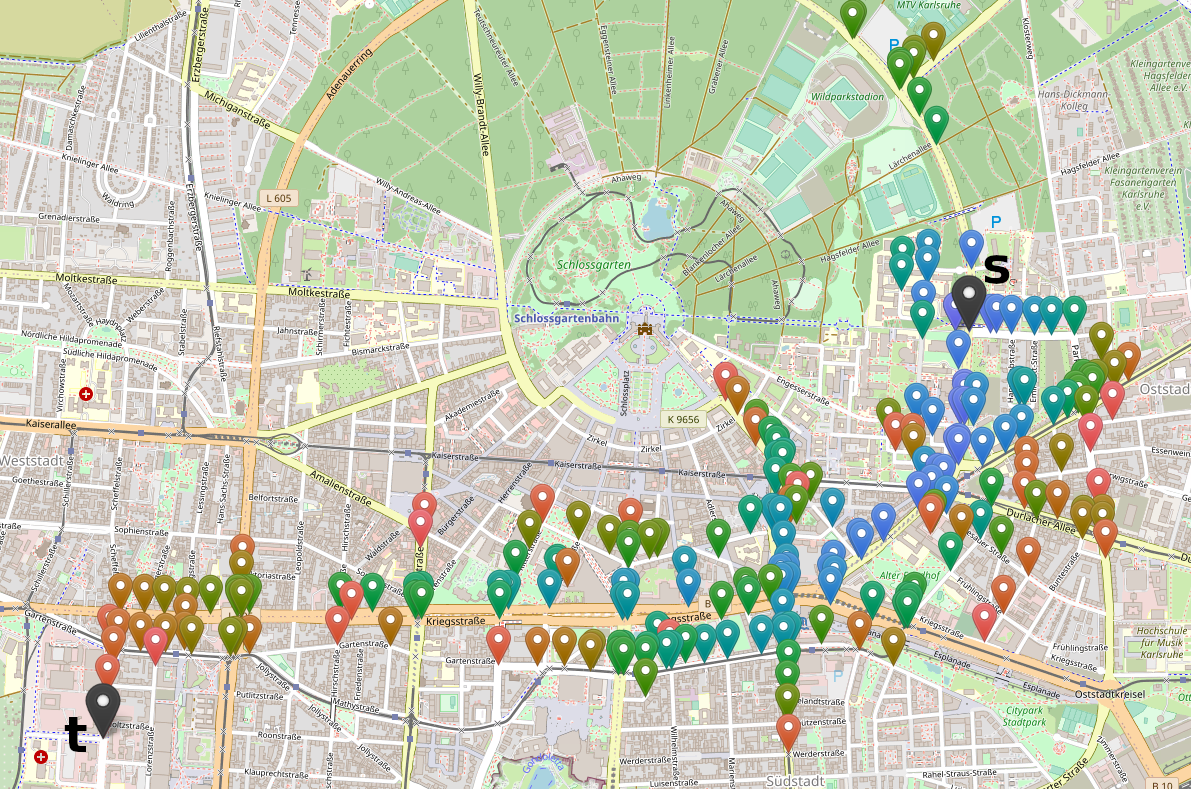
\includegraphics[width=.6\columnwidth]{fig/searchspace_st.png}
\caption{Nodes explored by A*. Color indicates the node removal order from the queue. Blue was removed first. Next is green. Red was removed last.}
\label{img:search-space}
\end{figure}

Unfortunately, for many real world applications, this basic graph model is too simplistic.
For realistic routing, many additional features need to be considered.
This includes turn costs and restrictions, live traffic, user preferences, and traffic predictions. %, temporary driving bans for certain types of vehicles.
Some applications may have additional application-specific requirements.
Extending Dijkstra's algorithm to support these features is usually easy.
Extending hierarchical speed-up techniques is also possible.
However, the algorithm development is vastly more complex.
For every feature, dedicated research paper(s) exist that extend CH.
Supporting the combination of several features is even harder.
For example, we are not aware of any work combining all features mentioned above.
In this paper, we describe an algorithmic building block, that allows handling the combination of all above mentioned features -- and probably more.

Our approach decouples extensions from the hierarchical speed-up technique by utilizing the A* algorithm~\cite{hnr-afbhd-68}.
A* is a goal-directed variant of Dijkstra's algorithm.
See Figure~\ref{img:search-space} for an example of nodes traversed during an A* search.
A* uses a \emph{heuristic} to guide the search towards the goal.
A heuristic is function that maps a node to an estimate of the remaining distance to the goal.
A*'s running time crucially depends on how tight this estimate is.
Further, evaluating the heuristic must be fast.
% The free flow travel time to the goal is a valid heuristic for most features.
% In many settings, it is the tightest lower bound available during preprocessing, i.e., independent of real-time data and user settings.
% However, to be useful we must be able to evaluate the free flow heuristic \todo{ist free flow heuristic besser als tight heuristic?} quickly and exactly.
In this paper, we describe CH-Potentials, a fast heuristic with tight estimates.
Internally, the heuristic uses a CH.
Fortunately, this is an implementation detail from the perspective of the A*.
To support a new feature, we only need to modify the A* algorithm.
The heuristic core containing the CH remains untouched.
Extending A* is vastly easier than extending a CH.
This enables us to design algorithms for a multitude of features.
In addition, we describe query optimizations for handling of low-degree nodes, common in road networks.
These low degree optimizations are applicable to Dijkstra's algorithm and A*.

The rest of the paper is organized as follows.
In Section~\ref{sec:related_work}, we discuss related works on goal directed search and extensions for realistic applications for hierarchical techniques.
CH-Potentials, our new distance estimation function is introduced in Section~\ref{sec:main-algo}.
Section~\ref{sec:low-deg-improvment} discusses our improvements for the handling of low-degree nodes.
In Section~\ref{sec:extensions}, we demonstrate CH-Potential's flexibility, by describing how to apply the approach to different practical applications.
Finally, in Section~\ref{sec:experiments}, we present an experimental evaluation of our approach.

\section{Related Work}\label{sec:related_work}

There is a lot of work that extends hierarchical speed-up techniques to more complex settings~\cite{bdgmpsww-rptn-16}.
For example, in~\cite{gv-errnt-11} turn information is integrated into CH.
The proposed approach achieves fast queries but preprocessing becomes an order of magnitude slower compared to classical CH.

A considerable amount of research and engineering effort has been put into studying the combination of traffic predictions with CH.
Several papers~\cite{bdsv-tdch-09,bgns-tdcha-10,klsv-dtdch-10,bgsv-mtdtt-13} and an entire dissertation~\cite{b-tdrpc-14} have been published on the subject.
Different variants with trade-offs regarding exactness, query speed and space consumption were proposed~\cite{bgsv-mtdtt-13}.
Recently, a new approach has been published~\cite{swz-sfert-20} which simultaneously achieves competitive results in all three aspects but only at the cost of considerable implementation complexity.

CRP~(Customizable Route Planning)~\cite{dgpw-crprn-13} is an engineered variant of MLD~\cite{swz-umlgt-02} which was developed to allow updating weights without invalidating the entire preprocessing.
For this, a faster, second preprocessing phase is introduced.
It can be run regularly to update weights.
In theory, this enables the integration of live traffic and user preferences.
In practice, live traffic feed data is imperfect.
Computing ``good'' routes without undesired detours due to artifacts in the data requires additional algorithmic extensions~\cite{dss-tarrn-18}.
CRP also supports turn costs.
Integrating traffic predictions into CRP was studied in~\cite{bdpw-dtdrp-16}.
On continental sized networks, TD-CRP can only compute approximate shortest distances (rather than paths).

In~\cite{dsw-cch-15}, CH is extended to Customizable CH (CCH).
CCH also has a second preprocessing phase where weights can be altered.
Supporting turn costs in CCH was studied in~\cite{bwzz-cchtc-20}.
% Turn integration still causes a slowdown of at least factor three to the second preprocessing phase.

Other extensions studied include electric vehicle routing~\cite{DBLP:journals/algorithmica/BaumDPSWZ20,DBLP:conf/aaai/EisnerFS11} or multi-criteria optimization~\cite{fns-opca-14,gks-rpfof-10}.

Another feature which has received quite some attention is the computation alternative routes~\cite{bdgs-argrn-11,adgw-arrn-13}.
Even formally defining what makes a good alternative route is non-trivial~\cite{bdgs-argrn-11}.
A variety of paradigms exists.
Competitive approaches require careful adjustment of their respective hierarchical speedup technique for the targeted paradigm.
In~\cite{krs-eepma-13}, the CRP customization is utilized to repeatedly compute shortest paths on graphs with slightly modified weights.
In~\cite{k-hdara-13}, partial shortest path trees are extracted from CH search spaces to find via-node candidates for alternative routes.
In~\cite{barth2019alternative}, a multi-criteria CH is extended to compute alternative routes with regards to multiple edge weight functions.

While these works show that it is possible to extend hierarchical approaches, they also show that it is non-trivial.
Further, in every extension the flexibility available at query time is fairly limited.
Combining these hierarchical extensions is an unsolved problem.

CH-Potentials is not the first work to combine hierarchical approaches and A*~\cite{bdsssw-chgds-10,gkw-blwr-07,bdgwz-sfpcs-19}.
However, previous works mostly focused on accelerating hierarchical approaches further rather than exploiting A*'s flexibility.

ALT~\cite{gh-cspas-05,gw-cppsp-05} and CPD-Heuristics~\cite{DBLP:conf/ijcai/BonoGHS19} are the two techniques with high conceptual similarity to CH-Potentials.
% Just as our approach, ALT is A*-based.
ALT has been combined with shortcuts~\cite{bdsssw-chgds-10} and also extended for dynamic graphs~\cite{dw-lbrdg-07} and time-dependent routing~\cite{ndls-bastd-12,dn-crdtd-12}.
% However, ALT's heuristic is not preprocessing-tight.
%
CPD-Heuristics are a combination of A* and Compressed Path Databases (CPD).
A CPD can quickly compute the first edge of a shortest path between any two nodes.
In~\cite{DBLP:conf/ijcai/BonoGHS19}, SRC~\cite{DBLP:conf/socs/StrasserHB14} is used as CPD.
For every distance estimation, a shortest path to the target is computed, whose length is used as the heuristic value.
Unfortunately, the employed CPD's quadratic preprocessing running time is problematic on large street networks.
%
% MtsCopa~\cite{DBLP:journals/tciaig/BaierBHH15} uses a similar idea to CPD-Heuristics but is only applied in a hunter-prey application.
%
In~\cite{DBLP:conf/ijcai/0002UJAKK18} the weighted graph is embedded into Euclidean space using FastMap. % such that distances in space and distances in the graph roughly correspond.
The Euclidean distance is then used as a distance estimate for A*.
% This results in a good but not a preprocessing-tight heuristic.


\section{Preliminaries}\label{sec:preliminaries}

We consider directed graphs $G=(V,E)$ with $n=|V|$ nodes and $m=|E|$ edges with weight functions $w : E \to \mathbb{R}$.
Given nodes $s$ and $t$ we want to obtain the path $P=(s=v_0,\dots,t=v_k)$ of minimal weight $w(P) := \sum_{i} w(v_{i-1}v_i)$.
We denote this shortest path weight as the distance $\dist_w(s,t)$ between $s$ and $t$.

\subsection{Dijkstra's Algorithm}

Dijkstra's algorithm~\cite{d-ntpcg-59} can be used to solve this point to point shortest path problem.
It maintains an array of tentative distances $d$ and a priority queue of nodes ordered by increasing distance from $s$.
Initially, all distances are set to $\infty$.
The start node distance $d[s]$ is set to zero and the queue initialized with $s$.
Then, in each iteration, the closest remaining node $u$ is popped from the queue and \emph{settled}.
Outgoing edges $uv$ are relaxed, i.e. $d[v] = \min(d[v], d[u] + w(uv))$.
If the distance at the head node $v$ was improved it will be inserted into the queue or the queue position will be updated if $v$ was already in the queue.
Once $t$ was settled, $d[t]$ contains the distance between $s$ and $t$.

Dijkstra's algorithm can also be run from the target $t$ on the reversed graph.
We call this a \emph{backward search}.
Running two Dijkstra searches, one from $s$ and a backward search from $t$, until the searches meet is called a \emph{Bidirectional Dijkstra}.
Typically, the searches are interleaved by alternating settling a node from each direction.
Another common approach is to always settle a node from the direction with the smaller minimal queue key.
Theoretically any direction interleaving strategy is possible.
The searches can also be run in parallel in two threads.
When the sum of the minimum keys in both queues $\overrightarrow{k} + \overleftarrow{k}$ is greater than the so far best known tentative total distance $\mu$ the algorithm can terminate.

\subsection{A*}\label{sec:a_star}

A* is a goal-directed variant of Dijkstra's algorithm.
% A* uses a \emph{heuristic} to guide the search towards the goal.
It uses a heuristic function $h_t(v)$ that maps a node $v$ onto an estimate of the distance from $v$ to the target.
The priority queue is ordered by $d[v] + h_t(v)$.
Thus, nodes closer to the target a explored earlier.

A* is equivalent to running Dijkstra's algorithm on the graph with \emph{reduced weights}~\cite{hnr-afbhd-68}.
This reduced weight function is defined as $w_{h_t}(uv) := w(uv) - h_t(u) + h_t(v)$.
A heuristic function is called \emph{feasible} if $w_{h_t} \geq 0$ for all edges.

\subsection{Contraction Hierarchy (CH)}

\begin{algorithm2e}
\KwData{$B[x]$: tentative distance from $x$ to target $t$}
\KwData{Min. priority queue $Q$, also called open list}
$B[x] \leftarrow +\infty$ for all $x\neq t$;
$B[t] \leftarrow 0$\;
Make $Q$ only contain $t$ with weight $0$\;
\While{not $Q$ empty}{
	$y\leftarrow$ pop minimum element from $Q$\;
	\For{$xy$ is down-edge in $G^+_\ell$}{
		\If{$B[x] > w_\ell(xy) + B[y]$}{
			$B[x]\leftarrow w_\ell(xy) + B[y]$\;
                        Add $x$ or decrease $x$'s key in $Q$ to $B[x]$\;
		}
	}
}
\caption{CH backward search}
\label{algo:ch-backward}
\end{algorithm2e}

\begin{figure}
\centering
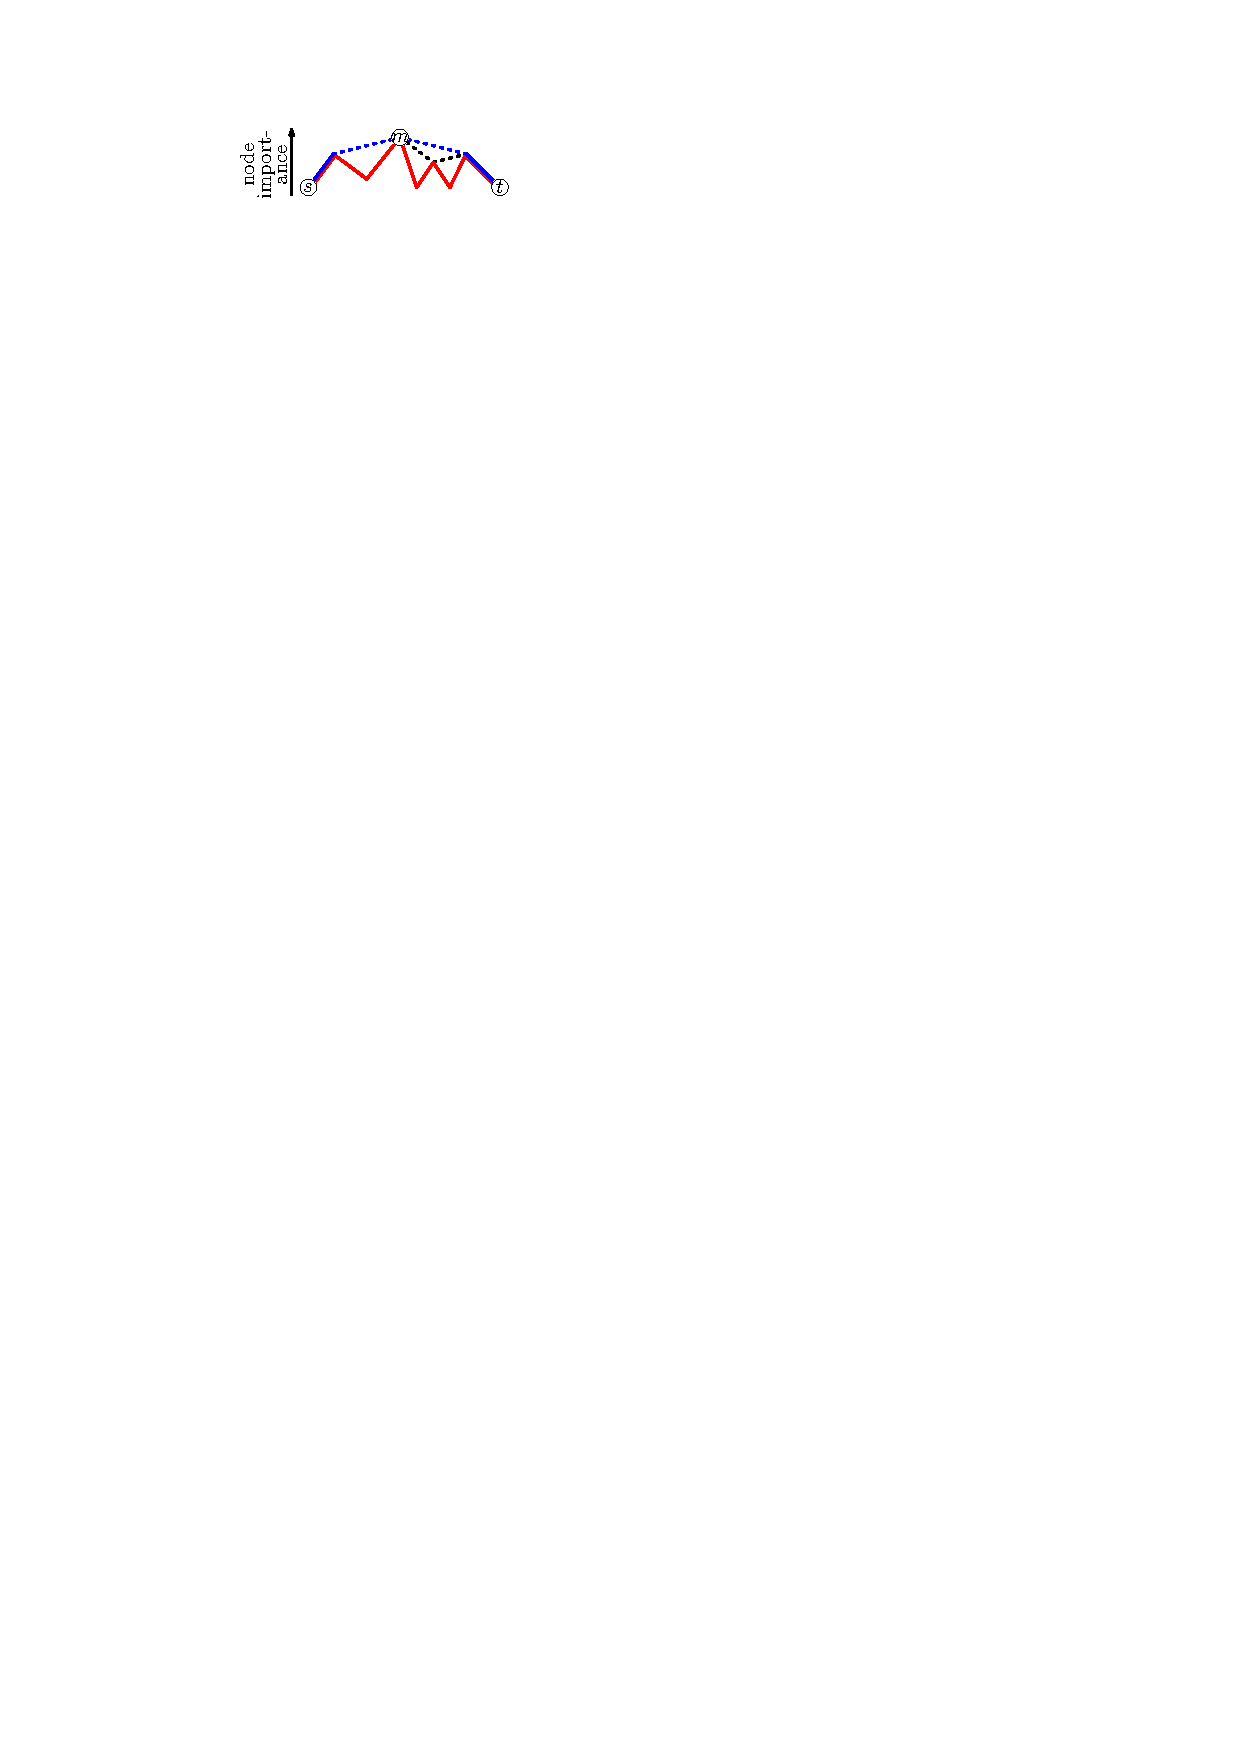
\includegraphics{fig/ch}
\caption{
Solid lines are edges in $G$. Dotted lines are shortcuts. Red is shortest $st$-path in $G$. Blue is equaly long up-down $st$-path in $G^+$. $m$ is the mid node.
}
\label{fig:ch}
\end{figure}

A CH is a two phase technique to efficiently compute exact, shortest paths.
For details, we refer to \cite{gssv-erlrn-12,dsw-cch-15}.
In this section, we give an introduction.

A CH places nodes into levels.
No edge must connect two nodes within one level.
Levels are ordered by ``importance''.
The intuition is that dead-ends are unimportant and at the bottom while highway bridges are very important and at the top.
An edge goes \emph{up} when it goes from a node in a lower level to higher level.
\emph{Down} edges are defined analogously.
An \emph{up-down path} is a path where only one node $m$ is more important than both its neighbors.
$m$ is called the \emph{mid} node.
An \emph{up path} is a path where the last node is the mid node.
Similarly, the first node is the mid node of a \emph{down path}.
% Every up and down path is an up-down path.
%
In the preprocessing phase, first, a node ordering is computed heuristically.
Then, \emph{shortcut} edges are added to the input graph $G$ to obtain $G^+$.
This is done by repeatedly contracting unimportant nodes and adding shortcuts between its neighbors.
%See~\cite{gssv-erlrn-12} for the details.
After the preprocessing, for every pair of nodes $s$ and $t$ there exists a shortest up-down $st$-path in $G^+$ with the same length as a shortest path in $G$.
See Figure~\ref{fig:ch} for a proof sketch.
From every shortest path (red) in $G$, an up-down path of equal length in $G^+$ (blue) exists.
Thus, we can restrict our search to up-down paths in $G^+$.
The search is bidirectional.
The forward search starts from $s$ and only follows up-edges.
Similarly, the backward search starts at $t$ and only follows down-edges in reversed direction.
The two searches meet at the mid node.
Pseudo-code for the backward search, i.e., the path from $m$ to $t$, is presented in Algorithm~\ref{algo:ch-backward}.
The forward search works analogously.
%
A CH query is fast, if the number of nodes reachable via only up- or down-nodes is small.
On road networks, this is the case~\cite{gssv-erlrn-12,dgpw-crprn-13}.
On graphs with low treewidth, this is also the case~\cite{dsw-cch-15,hs-gbpo-18}.

% Using the CH query algorithm, we can already give a simple heuristic.
% The heuristic evaluation $h_t(x)$ performs a CH-query from $x$ to $t$.
% This yields tight estimates but a high overhead for the heuristic evaluation.
% While a single CH query is fast, answering one for every node explored in the $A^*$ search is slow.
% Fortunately, we can do better.
% For this we need another component called PHAST~\cite{dgnw-phast-13}.

\subsection{Customizable Contraction Hierarchy (CCH)}

Customizable Contraction Hierarchies~\cite{dsw-cch-15} are a special variant of Contraction Hierarchies.
They use a node importance order independent of the weight function.
This allows splitting the preprocessing in two subphases.
The first one is slow but independent of the weight function.
The second one, called \emph{customization}, is fast (less than a second) and applies a weight function to the preprocessed data.
This allows regular updates to the weight function, for example to incorporate live traffic.

As for CH, the result of the preprocessing is an augmented graph $G^+$ fulfilling the same properties as for CH.
Thus, the CH query algorithms can be applied without modifications.
However, the CCH preprocessing grants some additional useful properties.
During preprocessing, an \emph{elimination tree} can be constructed.
The root of the elimination tree is the most important node.
For every other node its parent is its least important upward neighbor.
In~\cite{bcrw-s-16}, it was proven that set of ancestors of a node in the elimination tree is equal to the nodes reachable in a forward/backward CH search.
This makes it possible to explore the CCH search space with a more efficient shortest path algorithm for DAGs:
Traverse elimination tree from source and target to root node and for each node relax all up-edges (reversed down-edges for the backward search).
Because this algorithm does not require a queue, it is faster than a Dijkstra based CH query.

\subsection{PHAST}

\begin{algorithm2e}
\KwData{$P[x]$: tentative distance from $x$ to $t$}
Execute Algorithm~\ref{algo:ch-backward}\;
\For{all CH levels $L$ from most to least important}{
	\For{all up edges $xy$ in $G^+_\ell$ with $x$ in $L$}{
		\If{$P[x] < P[y] + w_\ell(xy)$}{
			$P[x] \leftarrow P[y] + w_\ell(xy)$\;
		}
	}
}
\caption{PHAST basic all-to-one search}
\label{algo:phast}
\end{algorithm2e}

PHAST~\cite{dgnw-phast-13} is a CH extension that computes distances from all nodes to one target node (or vice versa, the one-to-all case works analogously).
The preprocessing phase remains the same as for CH.
The query phase is split into two steps.
The first step is analogue to the CH query:
From $t$, all reachable nodes via reversed down-edges are explored.
Algorithm~\ref{algo:ch-backward} shows this first step.
The second step iterates over all CH levels from top to bottom.
In each iteration, all up-edges starting within the current level are followed in reverse.
After all levels are processed, the shortest distances from all nodes to $t$ were computed.
Pseudo-code is provided in Algorithm~\ref{algo:phast}.
PHAST is faster than Dijkstra's algorithm on road graphs because it is a better fit for modern processor architectures.
It can also easily be parallelized.
% However, we will not consider parallelization in this paper.
We refer to~\cite{dgnw-phast-13} for an in-depth experimental performance analysis.
% Using PHAST, we can also compute a tight A* heuristic.
% In the query phase, we first run PHAST to compute the distances from every node to $t$ with respect to $w_\ell$ and store the result in an array $H$.
% Next, we run $A^*$ and implement the heuristic as a lookup in the array $H$.

% This PHAST-based algorithm works.
% The $H$ lookup and by extension the $A^*$ search is indeed fast.
% However, the PHAST step before the search is comparatively expensive.
% The reason is that the distances towards $t$ are computed for \emph{all} nodes.
% Ideally, we only want to compute the distances from the nodes explored in the $A^*$ search.

\subsection{RPHAST}

RPHAST~\cite{delling_et_al:OASIcs:2011:3266}, short for Restricted PHAST, is a PHAST extension for efficiently computing distances from a smaller set of source nodes to one target node (again, the reversed case works analogously).
Given a set of source nodes $S$, the first step is to copy all up-edges reachable only through up-edges from the source nodes into a new graph.
This step is called \emph{selection}.
Then, in the query step a target $t$ is given and the PHAST algorithm is applied but the downward sweep (second step of the PHAST algorithm) is performed only on the restricted subgraph.
RPHAST is particularly effective when many targets are queried for the same source set $S$.
If the source set changes often, selection times may become problematic.

\section{The Incremental Many-to-One Problem}\label{sec:lazy-rphast}

Most route planning algorithms focus on the point-to-point shortest path problem.
However, certain applications need distances between sets $S$ and $T$ of nodes.
This is variant is known as the \emph{many-to-many} problem variant.
In some cases one of the sets is a single node.
This is then called a \emph{one-to-many} or \emph{many-to-one} problem.
RPHAST, as discussed in the previous paragraph, can be applied to these problems.

In this section, we discuss a very specific setting arises naturally from A* heuristics.
Here, the target node is known in the selection step but the source nodes are only queried one after another.
We denote this problem as the \emph{incremental many-to-one} problem.
The first step is the \emph{target selection} where the target node is provided.
Then, an arbitrary number of source nodes $s_i$ are given one after another and for each source the distance to the target has to be computed.

We consider the combined running time of the target selection and each incremental query as the total running time to answer an incremental many-to-one query.
Since the target selection time is included, computing the distances to all nodes with Dijkstra or PHAST is too slow.
Also, since the source set is only provided incrementally, RPHAST in its basic form is not well suited to our problem.
Fortunately, we can do better.

\subsection{Lazy RPHAST}

\begin{algorithm2e}
\KwData{$B[x]$: tentative distance from $x$ to $t$ as computed by Algorithm~\ref{algo:ch-backward}}
\KwData{$D[x]$: memoized distance final from $x$ to $t$, $\bot$ initially}
\SetKwFunction{Dist}{ComputeAndMemoizeDist}
\SetKwProg{Fn}{Function}{:}{}
\Fn{\Dist{$x$}}{
	\If{$D[x] = \bot$}{
		$D[x]\leftarrow B[x]$\;
		\For{all up edges $xy$ in $G^+_\ell$}{
                        $D[x]\leftarrow\min\{D[x],w_\ell(xy)+\Dist(y)\}$\;
		}
	}
	\Return{$D[x]$}\;
}
\caption{Lazy RPHAST algorithm}
\label{algo:pot}
\end{algorithm2e}

The core idea of our algorithm is to do the (R)PHAST computation lazily and using memoization as depicted in Algorithm~\ref{algo:pot}.
In the target selection, we first run the backward CH search from $t$ to obtain an array $B$.
$B[x]$ is the minimum down $xt$-path distance or $+\infty$, if there is no such path.
$B$ is computed as shown in Algorithm~\ref{algo:ch-backward}.

To compute the distance from a source $s_i$, we recursively compute for all up-edges $(s_i x)$ the distance $D[x]$.
Next, we compute the minimum distance over all up-down paths that contain at least one up-edge using $d = \min_x\{w_\ell(s_i x) + D[x]\}$.
As not all shortest up-down paths contain an up-edge, we set $D[s_i] = \min \{ B[s_i], d \}$.
This calculation is correct, as it computes the minimum up-down $s_it$-path distance in $G^+_\ell$, which corresponds to the minimum $s_it$-path distance in a CH.
% A* with this heuristic is the basic CH-Potentials algorithm.

\subsection{Lazy RPHAST on CCH}

Algorithm~\ref{algo:pot} can be applied to CCH without any modifications.
However, we can also exploit the elimination tree for the Lazy RPHAST algorithm.
Computing the distance $D[x]$ requires knowing the final distance of all upward neighbors.
In Algorithm~\ref{algo:pot} we have to compute these distances recursively.
All upward neighbors of $x$ are by definition included in the search space, thus they are also ancestors in the elimination tree.
If the distance of the parent in the elimination tree has already been computed, the distances of all other upward neighbors also has to have been computed.
Thus, it is sufficient to recursively (or iteratively) ensure that the distance of the parent in the elimination tree has been computed.
As soon as a node with final distance is encountered, all ancestors are known to have their final distance.
This allows for the more efficient implementation depicted in Algorithm~\ref{algo:cch_pot}.

\begin{algorithm2e}
\KwData{$B[x]$: tentative distance from $x$ to $t$ as computed by Algorithm~\ref{algo:ch-backward}}
\KwData{$D[x]$: memoized distance final from $x$ to $t$, $\bot$ initially}
\KwData{$P[x]$: parent node of $x$ in the elimination tree}
\SetKwFunction{Dist}{ComputeAndMemoizeDist}
\SetKwProg{Fn}{Function}{:}{}
\Fn{\Dist{$x$}}{
	\If{$D[x] = \bot$}{
		\If{$P[x] \neq \bot$ and $D[P[x]] = \bot$}{
			$\Dist(P[x])$\;
		}
		$D[x]\leftarrow B[x]$\;
		\For{all up edges $xy$ in $G^+_\ell$}{
                        $D[x]\leftarrow\min\{D[x],w_\ell(xy)+D[y]\}$\;
		}
	}
	\Return{$D[x]$}\;
}
\caption{Elimination tree based Lazy RPHAST algorithm}
\label{algo:cch_pot}
\end{algorithm2e}

\subsection{Many-to-Many with Lazy RPHAST}

In this section, we discuss how the Lazy RPHAST algorithm can be applied in a many-to-many context.
To the best of our knowledge, the fastest way to compute a full distance table between a set of sources and a set of targets is RPHAST utilizing SSE instructions to process several sources at once.
First, the selection phase is performed for the full target set.
Second, a query is performed for each source which yields the distances from this source to all targets (RPHAST).
This second step can be improved by processing $k$ (typically 16) sources at once using SIMD vector instructions (SSE RPHAST).

Since RPHAST is the fastest known algorithm for many-to-many computations, investing how well Lazy RPHAST performs in this setting appears to be an interesting question.
The naive approach would be to select one target after another and for each one doing the full lazy exploration from all sources.
However, this approach would explore the upward search space of all the sources over and over again.
This would not be competitive.

Luckily, we can do better by using a different One-to-Many CH variant -- the Bucket-CH algorithm~\cite{gssv-erlrn-12} -- to select all targets at once.
The Bucket CH selection phase works as follows:
For each node $x$, we maintain an initially empty list $B[x]$ of tuples $(t_i, dist(x,t_i))$, also called a \emph{bucket}.
These buckets can be populated by running a backward CH search (Algorithm~\ref{algo:ch-backward}) from each $t_i$ and inserting the resulting distances into the buckets.
Now we can utilize Algorithm~\ref{algo:pot} (or~ Algorithm~\ref{algo:cch_pot}) to compute distances from a given source to \emph{all} targets at once.
We only have to change $D[x]$ so that it is an array of distances to each $t_i$ instead of a single scalar value.
After calling the adjusted \texttt{ComputeAndMemoizeDist} for each source, we know the shortest distances between each pair of source and target node.
This way, we explore the search space of the sources only once.

The Bucket-CH selection phase still explores the shared parts of the search space of the targets several times.
This can also be improved with the following modified CH backward search:
All target nodes are inserted into the queue at once.
The priority queue is ordered by importance instead of distance.
Distance labels are buckets instead if scalar values.
The buckets of each target node are initialized with a single entry for the respective node with distance zero.
When relaxing an edge, the bucket of the head nodes is merged with the bucket of the tail node with each distance increased by the weight of the edge.
By keeping the buckets sorted, this merging can be efficiently implemented with a coordinated linear sweep over both buckets.
We evaluate our Lazy RPHAST many-to-many algorithm with this improved Bucket-CH selection in Section~\ref{todo}.

\section{A* with CH-Potentials}\label{sec:main-algo}

In this section, we describe how to use the Lazy RPHAST algorithm to build a fast and tight heuristic for A*.
We also discuss CH-Potentials for the bidirectional A* algorithm and propose an improved pruning criterion for symmetric bidirectional potentials.
Further, we present several low degree node optimization which exploit road network characteristics to reduce the overhead of queue operations and heuristic evaluations.
Finally, we introduce an algorithmic framework to apply A* with CH-Potentials to a variety of practical route planning problems.

The CH-Potentials heuristic is a straightforward application of the Lazy RPHAST algorithm.
In the beginning of each query, we perform the target selection, a backward CH search, from the target $t$.
The heuristic function $h_t(x)$ is implemented by a call to the \texttt{ComputeAndMemoizeDist} for node $x$.

This yields a \emph{perfect} heuristic, at least as long as the CH preprocessing and the A* algorithm are performed on the same graph with the same weight function.
This case is of course not particularly interesting.
One could just answer the shortest path query directly with a CH query.
This approach becomes useful when the query runs on a \emph{different but related} graph or weight function than the preprocessing.
We will discuss such applications in Section~\ref{sec:extensions}.
But before that, we discuss two extensions/optimizations to A* which we will utilize.

\subsection{Low Degree A* Improvements}\label{sec:low-deg-improvment}

Preliminary experiments showed, that a significant amount of query running time is spent in heuristic evaluations and queue operations.
We can reduce both by keeping some nodes out of the queue, as the heuristic needs to be evaluated when a node is pushed into the queue.
Avoiding pushing low degree nodes into the queue is the focus of this section.
The techniques discussed here are a lazy variant of the ideas used in TopoCore~\cite{DBLP:conf/gis/DibbeltSW15}.

We modify A* by processing low degree nodes consecutively without pushing them into the queue.
Our algorithm uses the undirected degree $d(x)$ of a node $x$.
Formally, $d(x)$ is the number of nodes $y$ such that $(xy)\in E$ or $(yx)\in E$.

Analogous to A*, our algorithm stores for every node $x$ a tentative distance $D[x]$.
Additionally, it maintains a minimum priority queue.
Diverging from A*, not all nodes can be pushed but every node has a tentative distance.

\subsubsection{Skip Degree Two Nodes}

Our algorithm differs from A* when removing a node $x$ from the queue.
A* iterates over the outgoing arcs $(xy)$ of $x$ and tries to reduce $D[y]$ by relaxing $(xy)$.
If A* succeeds, $y$'s weight in the queue is set to $D[y]+h_t(y)$.
Our algorithm, however, behaves differently, if $d(y)\le 2$.
Our algorithm determines the longest degree two chain of nodes $x y_1,\ldots, y_k, z$ such that $d(y_i)=2$ and $d(z) > 2$.
If our algorithm succeeds in reducing $D[y_1]$, it does not push $y_1$ into the queue.
Instead, it iteratively tries to reduce all $D[y_i]$.
If it does not reach $z$, then only $D$ is modified but no queue action is performed.
If $D[z]$ is modified and $d(z)>2$, $z$'s weight in the queue is set to $D[z]+h_t(z)$.

As the target node $t$ might have degree two, our algorithm cannot rely on stopping, when $t$ is removed from the queue.
Instead, our algorithm stops as soon as $D[t]$ is less than the minimum weight in the queue.

\subsubsection{Skip Degree Three Nodes}

We can also skip some degree three nodes.
Denote by $x y_1,\ldots, y_k, z$ a degree two chain as described in the previous section.
If $d(z) > 3$ or $z$ is in the queue, our algorithm proceeds as in the previous section.
Otherwise, there exist up to two degree chains $z a_1,\ldots,a_p b$ and $z,\alpha_1,\ldots,\alpha_q,\beta$ such that $a_1\neq y_k \neq \alpha_1$.
Our algorithm iteratively tries to reduce all $D[a_i]$ and $D[\alpha_i]$.
If it reaches $\beta$, $\beta$'s weight in the queue is set to $D[\beta]+h_t(\beta)$.
Analogously, if $b$ is reached, $b$'s weight is set to $D[b]+h_t(b)$.
If $b$ respectively $\beta$ are not reached, our algorithm does nothing.

\subsubsection{Stay in Largest Biconnected Component}\label{sec:largested-biconnected-component}

A lot of nodes in road networks lead to dead-ends.
Unless the source or target is in this dead-end, it is unnecessary to explore these nodes.

In the preprocessing phase, we compute the subgraph $G_C$, called \emph{core}.
$G_C$ is induced by the largest biconnected component of the undirected graph underlying $G$.
We do this using Tarjan's algorithm \cite{t-dfslg2-72}.
For every node $v$ in the input graph $G$, we store the attachment node $a_v$ to the core.
For nodes in the core, $a_v=v$.
We exploit that all attachment nodes are single node separators and the problem can be decomposed along them.

The query phase is divided into two steps.
In the first step, we apply A* with CH-Potentials to $G_C$ combined with the component that contains $s$.
This can be achieved implicitly by removing edges from $G_C$ into other components during preprocessing.
If $t$ is part of $G_C$ or in the same component as $s$, this A* search finds it.
Otherwise, we find $a_t$.
In that case, we continue by searching a path from $a_t$ towards $t$ restricted to $t$'s biconnected component.
The final result is the concatenation of both paths.

\subsection{Bidirectional A*}

Since bidirectional search provides an easy way to halve the running time of Dijkstra's algorithm, a bidirectional variant of A* also seems desirable.
However, as pointed out in~\cite{gh-cspas-05}, this is not as straightforward as one might expect.
One would like to use a forward potential $\overrightarrow{h}_t$ in the forward search and a backward potential $\overleftarrow{h}_s$ (computing distances in the reversed graph) in the reverse search.
The problem is that these two potentials induce different reduced graphs (see Section~\ref{sec:a_star}).
Thus, in the equivalent bidirectional Dijkstra search each direction would use different graph.
This would break the bidirectional Dijkstra stopping criterion.
To the best of our knowledge, no better stopping criterion exists than running \emph{both} searches until their minimum queue key $k$ becomes greater than the best known total tentative distance $\mu$.
But this is the same stopping criterion that a unidirectional A* search has.
Thus, this straightforward bidirectional A* performs about twice the work than a unidirectional A*.
This can be slightly improved by introducing pruning.
Nodes, for which $\overrightarrow{D}[x] + h(x) > \mu$ holds, i.e. their distance plus the estimate of the remaining distance is already greater than the currently known tentative distance, can not contribute to a shorter path and need not to be added to the queue.
This approach is denoted as the \emph{symmetric} bidirectional A*.

To overcome this problem the authors of propose the \emph{average} potential, a combined heuristic, which is good for both directions but also makes both searches run on the same reduced graph and thus enables an efficient stopping criterion.
The reduced graph of the average potential is the graph with the average weights of the reduced graphs of the forward and backward potentials.
The potential function which induces this average reduced graph is $h_{\overline{st}}(x) := \frac{\overrightarrow{h}_t(x) - \overleftarrow{h}_s(x)}{2}$ (and $-h_{\overline{st}}(x)$ for the backward search).
This potential allows stopping the searches when $\overrightarrow{k} + \overleftarrow{k} \geq \mu$.
Additionally, the pruning from the symmetric approach can be utilized with the original potentials.
To the best of our knowledge, this method is the fastest known variant of bidirectional A*.
Still, it has two downsides.
First, evaluating the average potential requires evaluating the original heuristics for both directions.
This can cause some overhead depending on the heuristics.
Second, for each direction on its own, the average potential is a worse heuristic than the original heuristic.

We propose an improved pruning criterion for the symmetric approach.
It takes the search progress (in form of the growing minimal queue keys) into account to tighten the pruning with increasing search progress and compensates for the worse stopping criterion.
As our experiments show, this makes the simpler symmetric approach at least competitive and sometimes even faster than the average potential.
Recall that the queue is ordered by $D[x] + h(x)$.
We use the minimal queue key $\overleftarrow{k}$ of the backward search to obtain a tighter estimate of $\dist(x,t)$.
If a node $x$ was not yet settled by backward search then $\dist(x,t) \geq \overleftarrow{k} - \overleftarrow{h}_s(x)$.
Thus, in the forward search if $\overrightarrow{D}[x] + \overleftarrow{k} - \overleftarrow{h}_s(x) > \mu$, we do not need to push $x$ into the queue.
The pruning for the backwards search works analogously.

% TODO alternating directions

\subsection{Applications}\label{sec:extensions}

% A* is a flexible algorithm.
% Many extended problems can therefore be solved using the CH-Potentials framework.
We start by establishing a common formal framework for the use of CH-Potentials.
Then, we exemplary describe some extended routing problems and how to apply CH-Potentials to them.

\subsubsection{Formal Setup: Inputs, Outputs, and Phases}

We consider a variety different applications, with slightly different problem models.
The goal is always to quickly answer many shortest path queries.
For the purpose of describing our framework, we establish a shared notation:
Input to each query are nodes $s$ and $t$, and a graph $G_q$ with query weights $w_q$.
However, the precise formal inputs of the query and what exactly $w_q$ represents depends on the application.
In the simplest case, $w_q$ will be scalar edge weights.
However, this is not a requirement.
It can be any function that computes a weight for an edge.
This function can also take additional parameters from the state of the search.
For example, in the case of live-traffic, $w_q$ represents scalar edge weights.
However, values of $w_q$ might change between queries.
In the case of traffic predictions, $w_q$ is a function which maps the edge entry time to the traversal time and the query takes an additional departure time parameter.

To enable quick shortest path computations, we consider a two phase setup with an additional off-line preprocessing phase before the on-line query phase.
The input to the preprocessing phase is a graph $G_\ell$ with lower bound weights $w_\ell$ and a node mapping function $\phi$.
$w_\ell(e)$ must be a scalar value for every edge $e$ of $G_\ell$.
We require that $w_q(u v)$ is greater or equal to the shortest distance $\dist_\ell(\phi(u), \phi(v))$ from $\phi(u)$ to $\phi(v)$ in $G_\ell$. % with respect to $w_\ell$.
The output of the preprocessing is auxiliary data that enables an efficient heuristic function $h_t(x)$.
$h_t(x)$ is the exact distance from $\phi(x)$ to $\phi(t)$ in $G_\ell$.
In the applications considered in this paper, $w_\ell$ is always the freeflow travel time.

The query phase uses this heuristic in an A* search between nodes $s$ and $t$ on $G_q$ and $w_q$.
Unless stated otherwise, $G_q$ and $G_\ell$ are the same graph and only $w_q$ changes for the queries.
The exact implementation of this A* search depends on the application.
Our approach only provides the heuristic $h_t$ for the A* search.
In contrast, the preprocessing phase remains the same for all applications.

Our heuristic is always \emph{feasible}, i.e. $w_q(u v) - h_t(u) + h_t(v) \geq 0$ holds for all edges.
By requirement and because of the triangle inequality the following holds:
\[
w_q(u v) - h_t(u) + h_t(v) \geq \dist_\ell(\phi(u), \phi(v)) - \dist_\ell(\phi(u), \phi(t)) + \dist_\ell(\phi(v), \phi(t)) \geq 0
\]
Thus, A* will always determine the correct shortest distances.

\subsubsection{Avoiding Tunnels and/or Highways}
\label{sec:no-tunnel-highway}

Avoiding tunnels and/or highways is a common feature of navigation devices.
Implementing this feature with CH-Potentials is easy.
We set $w_\ell$ to the freeflow travel time.
If an edge is a tunnel and/or a highway, we set $w_q$ to $+\infty$.
Otherwise, $w_q$ is set to the freeflow travel time.

\subsubsection{Forbidden Turns and Turn Costs}
\label{sec:no-turns}

The classical shortest path problem allows to freely change edges at nodes.
However, in the real world, turn restrictions, such as a forbidden left or right turn, exist.
Also, taking a left turn might take longer than going straight.
This can be modeled using turn weights~\cite{gv-errnt-11,dgpw-crprn-13,bwzz-cchtc-20}.
% In this section, we first present the extended problem setting.
% Afterwards, we describe how it can be solved with CH-Potentials.
A \emph{turn weight} $w_t$ maps a pair of incident edges onto the turning time or $+\infty$ for forbidden turns.
For CH-Potentials, we use zero as lower bound for every turn weight in the heuristic.
Thus, the graph $G_\ell$ and weights $w_\ell$ for preprocessing is the unmodified input graph without turn weights.

% Ich bleibe bei v_i hier, damit keine Verwechselung mit den freien Variablen x,y,z gibt.
A path with nodes $v_1, v_2,\ldots v_k$ has the following \emph{turn-aware weight}: \[
w_\ell(v_1 v_2) + \sum_{i=2}^{k-1}  w_t(v_{i-1},v_i,v_{i+1}) + w_\ell(v_i v_{i+1})
\]
The objective is to find a path between two given edges with minimum turn-aware weight.
The first term $w_\ell(v_1, v_2)$ is the same for all paths, as it only depends on the source edge.
It can thus be ignored during optimization.

We solve this problem by constructing a \emph{turn-expanded} graph as $G_q$.
Edges in the input graph $G_\ell$ correspond to \emph{expanded nodes} in $G_q$.
For every pair of incident edges $x y$ and $y z$ in $G_\ell$, there is an \emph{expanded edge} in $G_q$ with expanded weight $w_t(x,y,z) + w_\ell(y z)$.
A sequence of expanded nodes in the expanded graph $G_q$ corresponds to a sequence of edges in the input graph $G_\ell$.
The weight of a path in $G_q$ is equal to the turn-aware weight of the corresponding path in $G_\ell$ minus the irrelevant $w_\ell(v_1,v_2)$ term.
Thus, the turn-aware routing problem can be solved by searching for shortest paths in $G_q$.

In this scenario, preprocessing and query use different graphs $G_\ell$ and $G_q$.
We define the node mapping function $\phi$ as $\phi(x y) = y$.
Obviously, $w_q(xy, yz) = w_t(x,y,z) + w_\ell(y z) \geq \dist_\ell(\phi(x y), \phi(y z))$ and this approach yields a feasible heuristic.
Sadly, the undirected graph underlying $G_q$ is always biconnected, if the input graph is strongly connected.
The optimization described in Section~\ref{sec:largested-biconnected-component} is therefore ineffective.
With this setup, CH-Potentials support turns without requiring turn information in the CH.

% To prove that $h'(x,y)$ is consistent, consider the turn-aware weight of a path $v_1,v_2\ldots v_k$ with $v_1=x$, $v_2=y$, $v_{k-1}=p$, and $v_k=q$.
% We can lower bound the expression as follows:
% \[
% \sum_{i=2}^{k-1} w_\ell(v_i,v_{i+1}) \le \sum_{i=2}^{k-1} \underbrace{w_t(v_{i-1},v_i,v_{i+1})}_{0\le} + \sum_{i=2}^{k-1} \underbrace{w_q(v_i,v_{i+1})}_{w_\ell(v_i,v_{i+1})\le}
% \]
% $\sum_{i=2}^{k-1} w_\ell(v_i,v_{i+1})$ is a $yq$-path length in $G$.
% It is no shorter than the shortest $yq$-path length in $G$, which is equal to $h(y)$.
% The heuristic is therefore a lower bound.
% It is consistent because it is derived from exact shortest paths in $G$ with $w_\ell$.

\subsubsection{Predicted Traffic or Time-Dependent Routing}
\label{sec:predicted-traffic}

The classical shortest path problem assumes that edge weights are scalars.
However, in practice, travel times vary along an edge due to the traffic situation.
% The primary reason is traffic.
Recurring traffic can be predicted by observing the traffic in the past.
It is common \cite{bgsv-mtdtt-13,bdpw-dtdrp-16,swz-sfert-20} to represent these predictions as \emph{travel time functions}.
An edge weight is no longer a scalar value but a function that maps the entry time onto the traversal time.
% Performing this prediction is outside of the scope of this paper.
% It is common to refer to routing with predicted traffic as \emph{time-dependent routing}.
% Again, we first formalize the extended problem setting and then describe our solution with CH-Potentials.

In this setting, the query weight $w_q$ is a function from $E\times \mathbb{R}$ to $\mathbb{R}^+$.
$w_q(e, \tau)$ is the travel time through edge $e$ when entering it at moment $\tau$.
The input to the extended problem consists of a source node $s$ and a target node $t$, as in the classical problem formulation.
Additionally, the input contains a source time $\tau_s$.
A path with edges $e_1,e_2\ldots e_k$ is weighted using $\alpha_k$, which is defined recursively as follows:\[
\begin{split}
\alpha_{1} & = w_q(e_1, \tau_s) \\
\alpha_{k} & = \alpha_{k-1} + w_q(e_1, \alpha_{k-1})
\end{split}
\]
The objective is to find a path to $t$ that minimizes $\alpha_k$.

If all travel time functions fulfill the \emph{FIFO property}, this problem can be solved using a straightforward extension of Dijkstra's algorithm \cite{d-aassp-69}.
The necessary modification to A* is analogous.
Without the FIFO property the problem becomes NP-hard \cite{or-tnp-89}.
% The FIFO property states that it is never beneficial to wait at a node before entering an edge.
The FIFO property states that it is not possible to arrive earlier by departing later.
Formally stated, the following must hold $\forall e\in E,\tau\in \mathbb{R},\delta\in \mathbb{R}^+: w_q(e, \tau) \le w_q(e, \tau+\delta) + \delta$.
Our implementation stores edge travel times using piece-wise linear functions.
The A* search uses the tentative distance $\tau$ at a node $x$ when to evaluating the travel time of outgoing edges $x y$.
This strategy is very similar to TD-ALT~\cite{ndls-bastd-12,dw-lbrdg-07}.

For the preprocessing, we set $w_\ell(e) = \min_\tau w_q(e,\tau)$, that is the minimum travel time.
% With this setup, we extended CH-Potentials to support time-dependent routing.
By keeping travel time functions out of the CH, we avoid a lot of algorithmic complications compared to~\cite{bgsv-mtdtt-13,bdpw-dtdrp-16,swz-sfert-20,dn-crdtd-12} which have to create shortcuts of travel time functions.

\subsubsection{Live and Predicted Traffic}
\label{sec:live-predicted-traffic}

Beside predicted traffic, we also consider live traffic.
Live traffic refers to the current traffic situation.
It is important to distinguish between predicted and live traffic.
Live traffic data is more accurate for the current moment than predicted data.
It is possible that it differs significantly from predicted traffic, if unexpected events like accidents happen.
% The predicted travel time along an edge was estimated in the past.
% Accidents are examples of such unexpected events.
However, just using live traffic data is problematic for long routes as traffic changes while driving.
At some point, one wants to switch from live traffic to the predicted traffic.
In this section, we first describe a setup with only live traffic and then combine it with predicted traffic.

To support only live traffic, we set $w_\ell$ to the freeflow travel time.
$w_q$ is set to the travel time accounting for current traffic.
As traffic only increases the travel time along an edge, $w_\ell$ is a valid lower bound for $w_q$.
In a real world application, values from $w_q$ could be updated between queries.
This is all that is necessary to apply CH-Potentials in a live traffic scenario.

To combine live traffic with predicted traffic, we define a modified travel time function $w_q$ that is then used as query weights.
Denote by $w_p(e,\tau)$ the predicted travel time along edge $e$ at moment $\tau$.
Further, $w_c(e)$ is the travel time according to current live traffic.
Finally, we denote by $\tau_{\mathrm{soon}}$ the moment when we switch to predicted traffic.
In our experiments, we set $\tau_{\mathrm{soon}}$ to one hour in the future.
We need to make sure that the modified travel time function fulfills the no-waiting property.
For this reason, we cannot make a hard switch at $\tau_{\mathrm{soon}}$.
Our modified travel time function linearly approaches the predicted travel time. % with a bounded slope.
%
Formally, we set $w_q(e,\tau)$ to $w_c(e)$, if $\tau \leq \tau_{\mathrm{soon}}$.
Otherwise, we check whether $w_p(e,\tau_{\mathrm{soon}}) < w_c(e)$ is true.
If it is the case, we set $w_q(e,\tau)$ to $\max\{w_c(e)+(\tau_{\mathrm{soon}}-\tau), w_p(e,\tau)\}$.
Otherwise, we set $w_q(e,\tau)$ to $\min\{w_c(e)-(\tau_{\mathrm{soon}}-\tau), w_p(e,\tau)\}$.
% We then run the algorithm of Section~\ref{sec:predicted-traffic} with $w_q$ as query weight.
In our implementation, we to not modify the representation of $w_p$ but evaluate the formulas above at each travel time evaluation.
We set $w_\ell$ again to the freeflow travel time.

With this setup, CH-Potentials support a combination of live and predicted traffic.
We did not make any modification, that would hinder a combination with other extensions.
Further adding tunnel and/or highway avoidance or turn-aware routing is simple.
This straight-forward integration of complex routing problems is the strength of the CH-Potentials.

\subsubsection{CCH Potentials}

Supporting live traffic is also possible with a three-phase setup:
A slow preprocessing phase, a faster \emph{customization} phase, and fast queries.
The customization phase is run regularly and incorporates updates to the weights into the auxiliary preprocessing data.
CRP~\cite{dgpw-crprn-13} and CCH~\cite{dsw-cch-15} follow this setup.
As discussed in Section~\ref{sec:lazy-rphast}, the Lazy RPHAST algorithm and thus CH-Potentials can also be used with a CCH.
In terms of our framework this would mean having a second preprocessing phase which allows updating $w_\ell$ to the current traffic situation.
Thus, with CCH-Potentials, we could also support a three-phase setup.
This could, for example, be used to combine live traffic with turn costs and restrictions.
One could also apply live traffic updates to $w_q$ immediately and only update $w_\ell$ once the difference between $w_\ell$ and $w_q$ grows too big or when some edge weight update would set $w_q < w_\ell$.
% For applications which allow for a three-phase setup, CCH-Potentials are likely a better choice for supporting live traffic.
% However, evaluating CCH-Potentials is beyond the scope of this paper.
% We focus on evaluating CH-Potentials as a simple building block in the two-phase setup.

\subsubsection{Alternative Routes with the Penalty Method}

Providing users with multiple alternative good routes to choose from is another relevant feature for practical routing applications.
The penalty method is an established framework for computing such alternative routes~\cite{bdgs-argrn-11,krs-eepma-13,pz-iarp-13,kobitzsch2015alternative}.
It computes an alternative graph instead of a set of alternative routes.
This graph is constructed iteratively.
In each iteration, a shortest path between $s$ and $t$ is computed.
This path (or certain parts of it) is then added to the alternative graph depending on certain quality criteria.
Finally, all edge weights of the path and possibly adjoined edges are penalized.
This is repeated until the current path is more than $1 + \epsilon$ times longer than the original distance or until certain other stopping criteria are fulfilled.

The running time of the penalty method is usually dominated by shortest path computations.
Since this boils down to computing shortest paths on $G_{\ell}$ with a few increased edge weights this seems like a natural fit for A* with CH-Potentials.
While the schema outlined above is conceptually simple, it leaves open quite a few details which may have a severe impact on performance.
In this work, we do not develop our own variant of the penalty method but aim to reproduce the configuration reported by Kobitzsch in his dissertation~\cite{kobitzsch2015alternative}.
To the best of our knowledge, this is the latest, most thoroughly engineered and evaluated iteration of the penalty method which also achieves the qualitatively best results.
While some details remain unclear from the description in~\cite{kobitzsch2015alternative}, luckily we could obtain the original implementation from the authors to fill in the remaining details.
Since we reproduce this exact configuration except for the shortest path algorithm, qualitative results should carry over and we can focus only on running times in our work.

For sake of keeping this section self-contained, we now briefly reiterate the details of our configuration.
The stretch limited to $\epsilon = 0.25$, i.e. for any path $P = (u,\dots,v)$ in the alternative graph $w(P) \leq (1+\epsilon) \cdot \dist(u,v)$.
Shortest path edges are penalized multiplicative with a factor of $\psi = 1.1$, i.e. when an edges was $k$ times on a shortest path its weight will be $w_q = w_{\ell}\cdot\psi^k$.
We also penalize edges incident to shortest paths with an asymmetric additive rejoin penalty.
An edge $uv$ where $u$ is on a shortest path but $v$ is not will get its weight increased by $\psi_r \cdot \dist_{w_{\ell}}(s,t) \cdot \frac{\dist_{w_q}(s,u)}{\dist_{w_q}(s,t)}$.
An edge $uv$ where $v$ is on a shortest path but $u$ is not will get its weight increased by $\psi_r \cdot \dist_{w_{\ell}}(s,t) \cdot \frac{\dist_{w_q}(v,t)}{\dist_{w_q}(s,t)}$.
$\psi_r$ is set to 0.01.
To avoid over-penalization, we count the times a \emph{node} was on a shortest path and do not apply penalties, when this number exceeds $k_{\max} := \lceil\log_{\psi}(1+\epsilon)\rceil + 2$.
Shortest paths are split into segments not yet contained in the alternative graph.
A segment is only added if it is long enough (at least $0.05 \cdot \dist_{w_{\ell}}(s,t)$) and does not violate the maximum stretch condition.
We terminate the algorithm when any of the following conditions becomes true:
\begin{itemize}
	\item All nodes on the current shortest path have been penalized $k_{\max}$ times.
	\item 10 ore more segments have been added to the alternative graph.
	\item The shortest path is longer than $(1+\epsilon) \cdot \dist_{w_{\ell}}(s,t)$ with respect to the original metric.
	\item The shortest path is longer than $(1+\epsilon) \cdot \psi + 2\psi_r \cdot \dist_{w_{\ell}}(s,t)$ with respect to the penalized metric.
\end{itemize}
The last two stopping criteria can both be utilized for additional pruning in the A*.
As a final optimization, we run the forward and backward search in parallel in two threads.

\subsubsection{Temporary Driving Bans}

Truck routing differs from car routing due to night driving bans and other restrictions.
In~\cite{kswz-erptd-p-20}, a preliminary version of CH-Potentials\footnote{
In~\cite{kswz-erptd-p-20}, CH-Potentials are used as a blackbox referring to an early ArXiv preprint~\cite{strasser2019perfect} of ours.
Our submitted paper is the finished version of the ArXiv preprint.
\cite{kswz-erptd-p-20} does not describe any of the contributions of this paper.
} is used for such a scenario.
The work considers time-dependent blocked edges and waiting at parking locations.
Further, a trade-off between arrival time and route quality is considered.

\section{Evaluation}

\label{sec:experiments}

\begin{table}
\centering
\caption{Instances used in the evaluation with preprocessing running times to construct a CH or CCH-Potential. With CCH-Potentials $w_{\ell}$ can be updated by rerunning Phase 2 again.}\label{tab:graphs}
\begin{tabular}{lrrrrr}
\toprule
 &                &                & \multicolumn{3}{c}{Preprocessing [s]} \\ \cmidrule(lr){4-6} & Nodes          & Edges          & \multirow{2}{*}{CH} & \multicolumn{2}{c}{CCH} \\ \cmidrule(lr){5-6} & $[\cdot 10^6]$ & $[\cdot 10^6]$ &                     & Phase 1 & Phase 2 \\
\midrule
OSM Germany   &       16.2 &       35.4 &                          298.7 &        1\,467.4 &          10.1 \\
DIMACS Europe &       18.0 &       42.2 &                          276.2 &        2\,480.9 &          12.4 \\
TDGer06       &        4.7 &       10.8 &                           59.2 &         331.7 &           2.7 \\
TDEur17       &       25.8 &       55.5 &                          293.9 &        2\,102.3 &          14.1 \\
TDEur20       &       28.5 &       60.9 &                          311.9 &        2\,219.5 &          15.2 \\
\bottomrule
\end{tabular}


\end{table}

In this section, we present our experimental evaluation.
Our benchmark machine runs openSUSE Leap 15.1 (kernel 4.12.14), and has 128\,GiB of DDR4-2133 RAM and an Intel Xeon E5-1630 v3 CPUs which has four cores clocked at 3.7\,Ghz and 4~$\times$~32\,KiB of L1, 8~$\times$~256\,KiB of L2, and 10\,MiB of shared L3 cache.
All experiments were performed sequentially.
Our code is written in Rust and compiled with rustc 1.47.0-nightly in the release profile with the target-cpu=native option.
The source code of our implementation and the experimental evaluation can be found on Github\footnote{\url{https://github.com/kit-algo/ch_potentials}}.

\subsection{Inputs and Methodology}
Our main benchmark instance is a graph of the road network of Germany obtained from Open Street Map\footnote{\url{https://download.geofabrik.de/europe/germany-200101.osm.pbf}}.
To obtain the routing graph, we use the import from RoutingKit\footnote{\url{https://github.com/RoutingKit/RoutingKit}}.
The graph has 16M nodes and 35M edges.
For this instance, we have proprietary traffic data provided by Mapbox\footnote{\url{https://mapbox.com}}.
The data includes a live traffic snapshot from Friday 2019/08/02 afternoon and comes in the form of 320K OSM node pairs and live speeds for the edge between the nodes.
It also includes traffic predictions for 38\% of the edges as predicted speeds for all five minute periods over the course of a week.
We exclude speed values which are faster than the freeflow speed computed by RoutingKit.
We also perform experiments on the Europe instance provided by PTV\footnote{\url{https://ptvgroup.com}} for the 9th DIMACs implementation challenge~\cite{DemetrescuGJ09}.
Additionally, we have three graphs with proprietary traffic predictions also provided by PTV.
The PTV instances are not OSM-based.
One is an old instance of Germany with traffic predictions from 2006 for 7\% of the edges and the other one a newer instance of Europe with predictions for 27\% of the edges.
% TODO PTV20
Table~\ref{tab:graphs} contains an overview over our instances.
In this table, we further include the sequential preprocessing running time to construct the (C)CH.
We report preprocessing running times as averages over 10 runs.
To evaluate point-to-point queries, we generate 10\,000 queries where both source and target are nodes drawn uniformly at random and report average results.
For many-to-one and many-to-many algorithms, we use the methodology from~\cite{delling_et_al:OASIcs:2011:3266}.
We generate a \emph{ball} $B$ of nodes around 100 uniformly at random chosen nodes by running a Dijkstra search until $|B|$ nodes are settled where $|B|$ is a parameter varied throughout the experiments.
From each ball we uniformly at random draw a set of sources $S$ and targets $T$ with $|S| = |T| = 2^{14}$.
For one-to-many experiments, we pick 100 sources of $S$ and for each source compute the distances to all nodes in the respective $T$ for a total of 10\,000 one-to-many queries.
For many-to-many experiments, we compute the distance table between the 100 $S$, $T$ pairs.

\subsection{Lazy RPHAST}

\begin{figure}
\centering
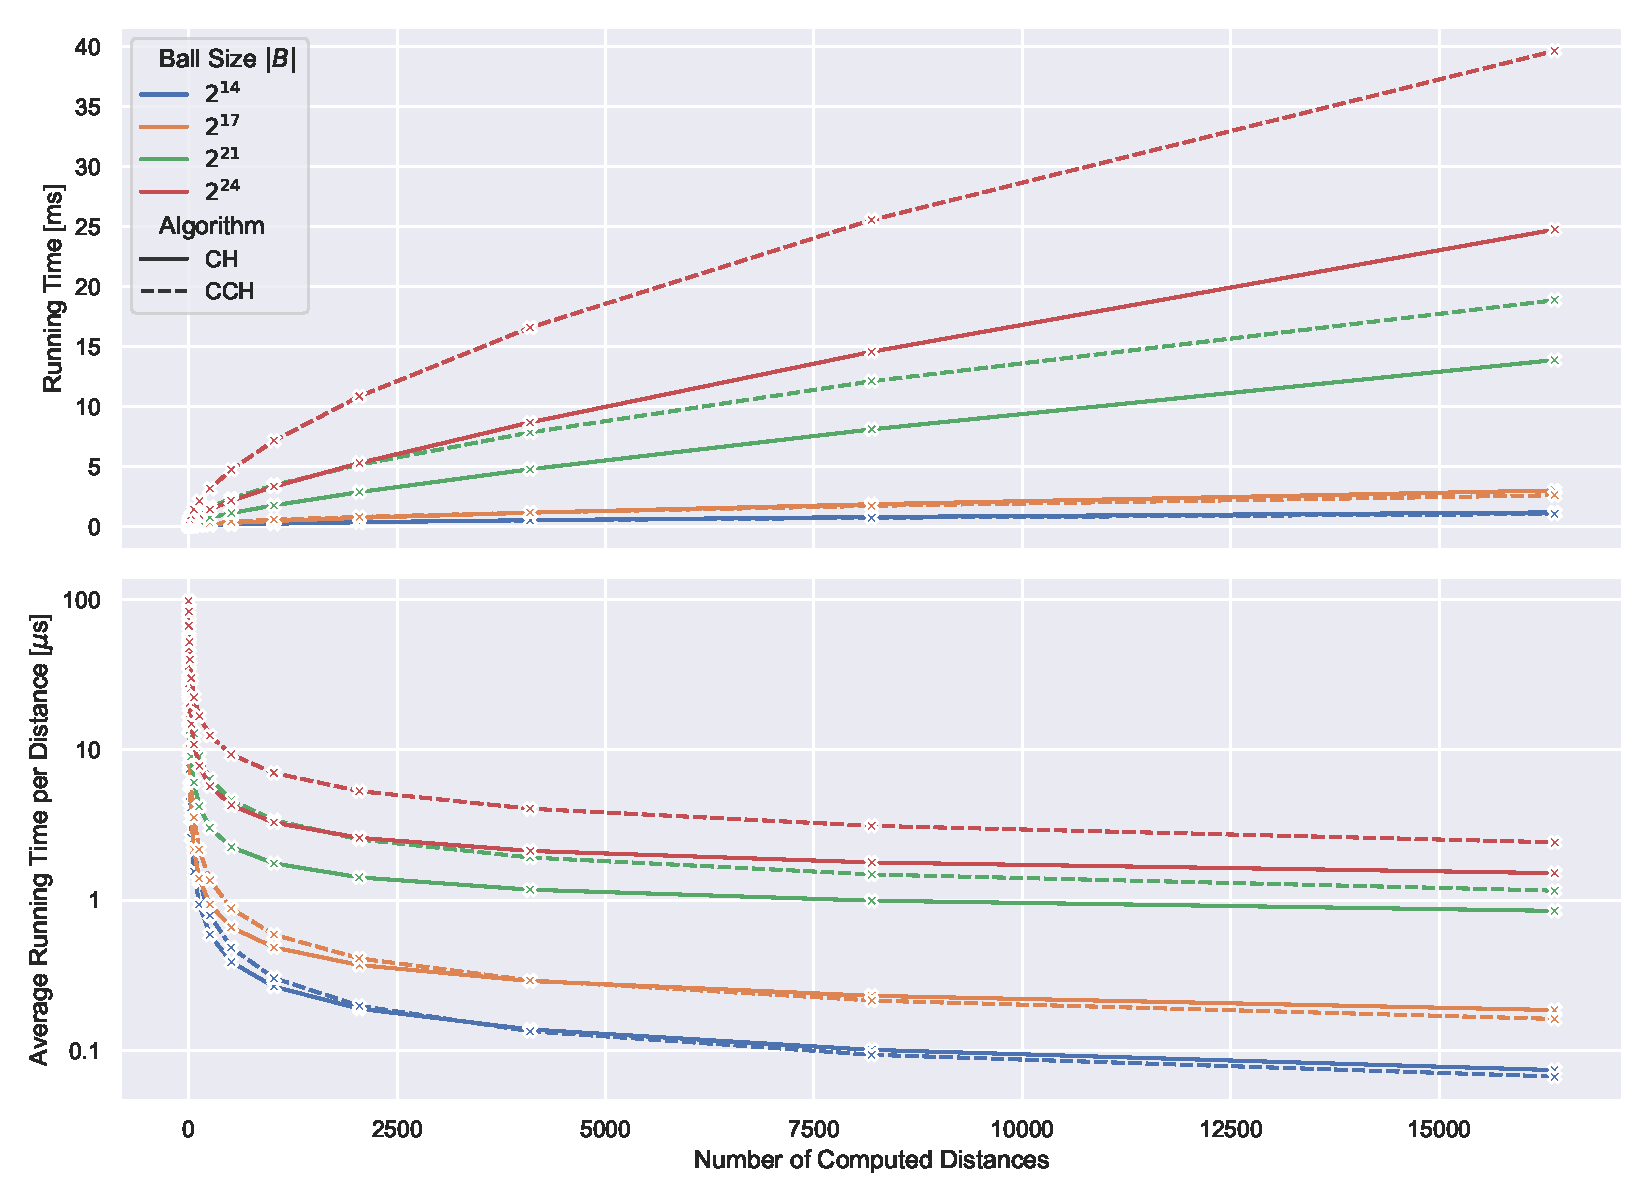
\includegraphics[width=\linewidth]{fig/lazy_rphast_inc.pdf}
\caption{
Total and per distance running times of incremental Lazy RPHAST with up to $|T| = 2^{14}$ targets picked from a ball of varying size $|B|$ on OSM Germany.
Note the different y-axis scales and units.
}\label{fig:lazy_rphast_inc}
\end{figure}

To evaluate Lazy RPHAST in the incremental setting, we measure the elapsed time after $2^i$ distances were computed.
Figure~\ref{fig:lazy_rphast_inc} depicts the total elapsed time and the average running time to compute a single distance.
The first few distances are the most expensive ones since a lot of the CH search space has not been explored yet.
For later queries, only little work remains to be done and the overhead per distance becomes basically a constant depending on the ball size.

The performance difference between the CH and CCH based variant is interesting.
The CCH based variant can utilize the elimination tree for a more efficient implementation but the search space denser.
This makes earlier queries more expensive and later queries cheaper.
With this trade-off, it depends on the ball size which variant is faster in terms of total running time.

\begin{figure}
\centering
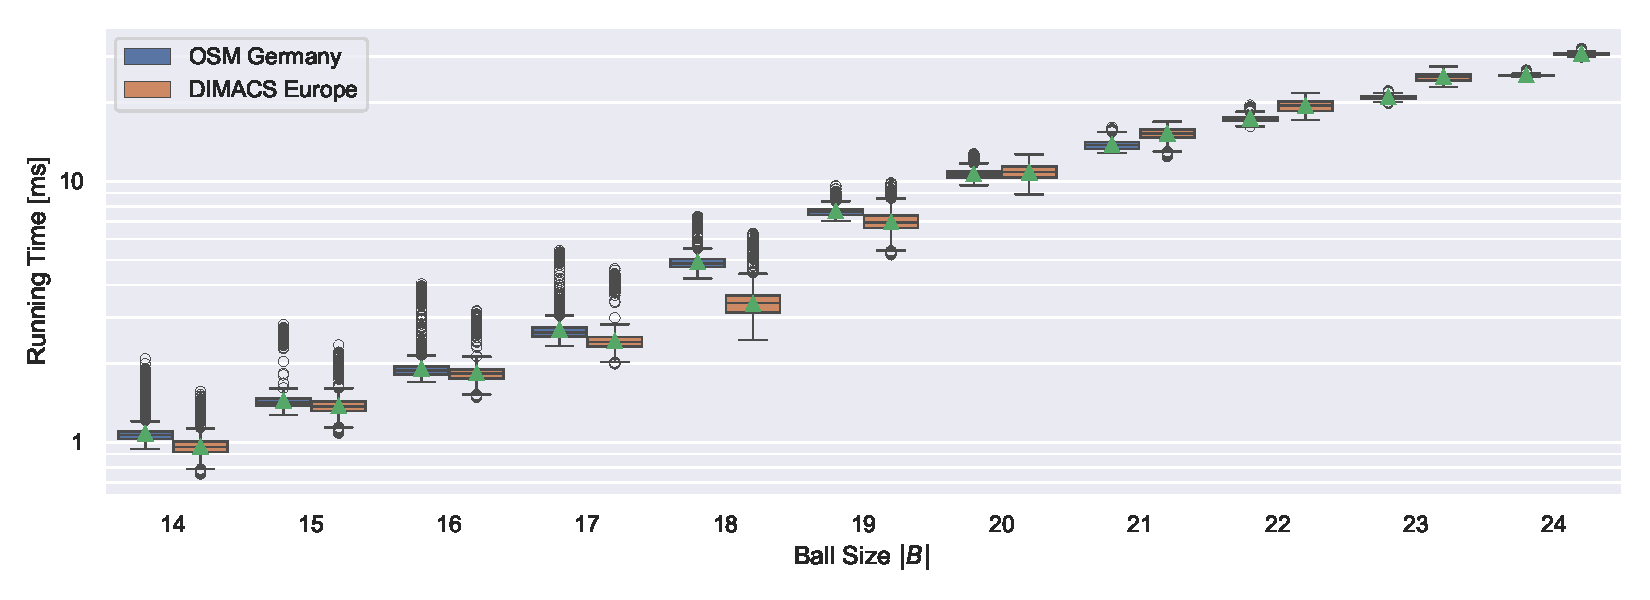
\includegraphics[width=\linewidth]{fig/lazy_rphast_many_to_one.pdf}
\caption{
Running times of CH based Lazy RPHAST with $|T| = 2^{14}$ targets picked from a ball of varying size $|B|$.
}\label{fig:many_to_one}
\end{figure}

\begin{figure}
\centering
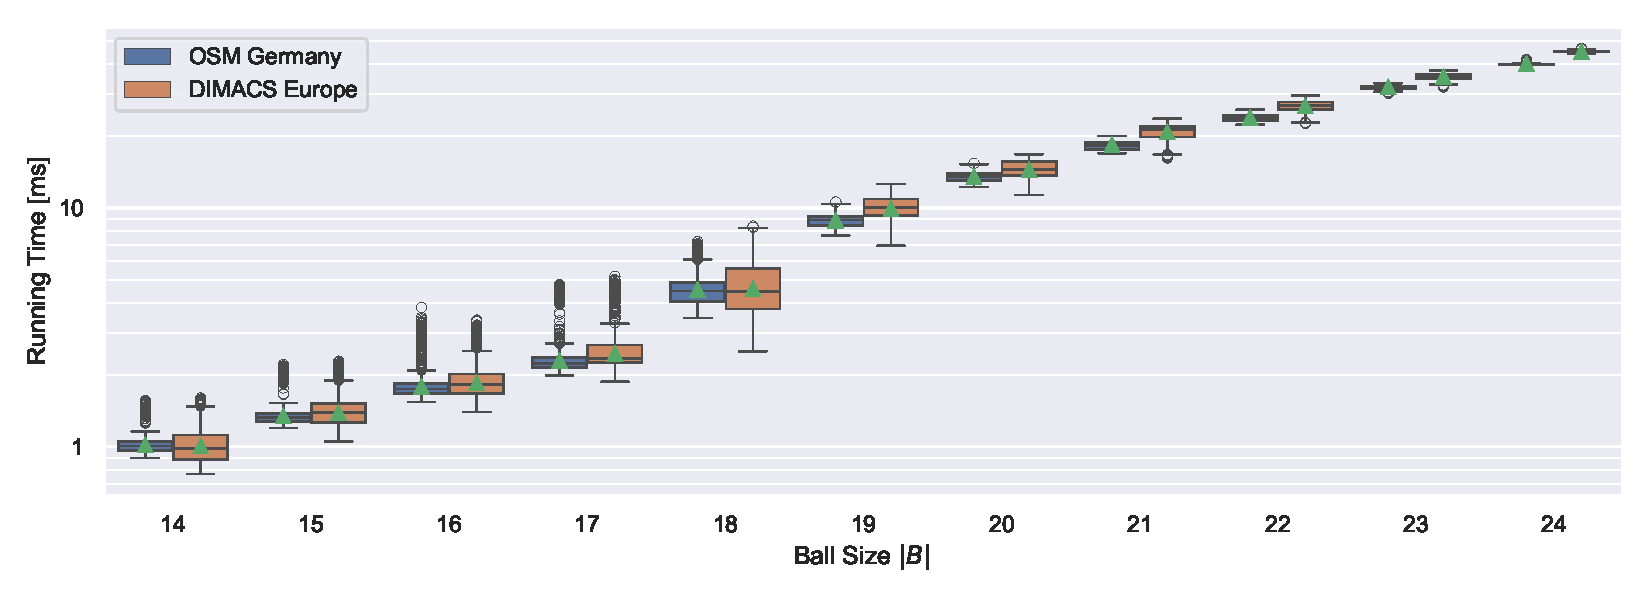
\includegraphics[width=\linewidth]{fig/lazy_rphast_cch_many_to_one.pdf}
\caption{
Running times of CCH based Lazy RPHAST with $|T| = 2^{14}$ targets picked from a ball of varying size $|B|$.
}\label{fig:many_to_one_cch}
\end{figure}

Despite the laziness being the distinguishing feature in Lazy RPHAST, the algorithm can still be used for non-incremental one-to-many queries.
Figures~\ref{fig:many_to_one} and~\ref{fig:many_to_one_cch} depict average running times to compute distances between one node and $2^{14}$ targets for different ball sizes.
This experiment uses the methodology exactly as described in~\cite{delling_et_al:OASIcs:2011:3266} which allows to relate our results to the performance of competing algorithms (set aside the performance differences caused by using a different test machine).
When looking at total running times for one source target set pair, Lazy RPHAST delivers very competitive performance and is as fast if not faster than all algorithms evaluated in~\cite{delling_et_al:OASIcs:2011:3266}
For example, Delling et al. report an average RPHAST running time of 1.97\,ms for selection and query combined for $|B| = 2^{14}$ and 28.52\,ms for $|B| = 2^{20}$ on DIMACs Europe.
Lazy RPHAST (on a CH) takes 0.96\,ms and 10.76\,ms respectively, to compute the same distances.
The CCH variant is slightly slower (1.00\,ms and 14.41\,ms) but still significantly faster than RPHAST.
This is of course not a fair comparison since the approaches in~\cite{delling_et_al:OASIcs:2011:3266} are geared towards having one expensive selection phase and than many faster query phases.
When computing distances from different source towards the same target set, RPHAST will outperform Lazy RPHAST.
However, whenever the target set may change between queries, Lazy RPHAST is a simpler and faster alternative.

\begin{figure}
\centering
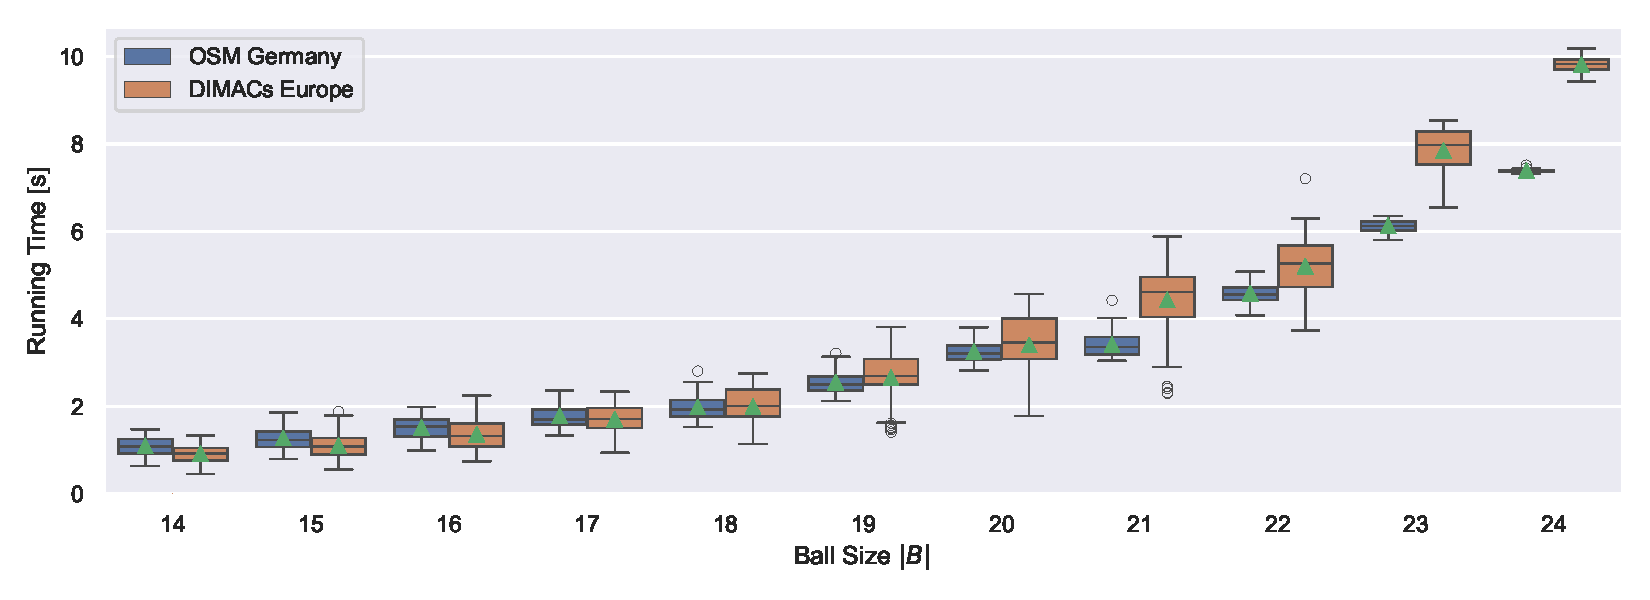
\includegraphics[width=\linewidth]{fig/lazy_rphast_many_to_many.pdf}
\caption{
Average running times of Lazy RPHAST for many-to-many queries with $|S| = |T| = 2^{14}$ sources and targets picked from a ball of varying size $|B|$ with standard deviation indicated as error bars.
The lower part of the bars indicates the running time of the Bucket CH subphase.
}\label{fig:many_to_many}
\end{figure}

Applying Lazy RPHAST to the many-to-many problem results in running times as depicted in Figure~\ref{fig:many_to_many}.
The results are again at least competitive to the performance reported for SSE RPHAST in~\cite{delling_et_al:OASIcs:2011:3266} which to the best of our knowledge is the fastest known approach.
The Bucket CH based first query phase takes between half of the time for $|B| = 2^{14}$ and a tenth of the time for $|B| = 2^{24}$.
It is worth noting that our approach does not require any explicit utilization of SSE instructions -- contrary to SSE RPHAST.
Nevertheless, an inspection of the generated assembly reveals that the code for Lazy RPHAST on an array of distances was automatically vectorized by the compiler.

\subsubsection{k-Nearest-Neighbor Queries with CCH}

One-to-many queries appear in many extended applications as a subproblem.
In some of these cases Lazy RPHAST can be used to achieve significant speed-ups with surprisingly little effort.
One such example are k-Nearest-Neighbor Queries with CCH~\cite{buchhold_et_al:LIPIcs.SEA.2021.18}.
There, shortest distances are computed repeatedly from the same source to boundary nodes of a cell of nodes.
On our suggestion, the authors integrated Lazy RPHAST into their algorithm which took only a couple of lines of code~\footnote{\url{https://github.com/vbuchhold/routing-framework/commit/c739dc8e81}}.
We reran their improved experiments and include the results in our appendix.
Briefly summarized, integrating Lazy RPHAST into this algorithm decreased running times by up to 15 times depending on the distribution of the target set for almost no effort.

\subsection{(C)CH-Potentials Heuristic}

\begin{figure}
\centering
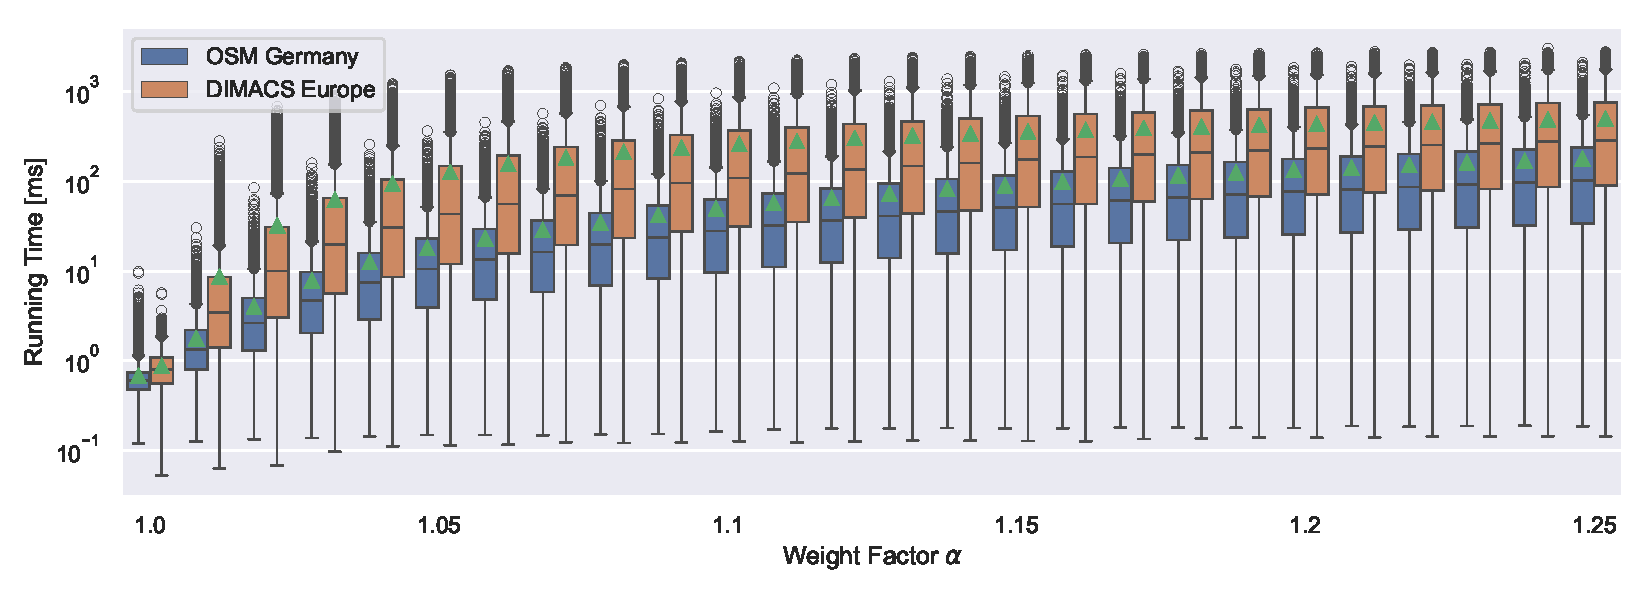
\includegraphics[width=\linewidth]{fig/scaled_weights.pdf}
\caption{
Running times on a logarithmic scale for queries on OSM Ger with scaled edge weights $w_q = \alpha \cdot w_\ell$.
The boxes cover the range between the first and third quartile.
The band in the box indicates the median, the diamond the mean.
The whiskers cover 1.5 times the interquartile range.
All other running times are indicated as outliers.
}\label{fig:scaled_weights}
\end{figure}

The performance of A* depends on the tightness of the heuristic and the overhead of evaluating the heuristic.
CH-Potentials computes optimal distance estimates with respect to $w_\ell$.
However, for most applications, there will be a gap between $w_q$ and $w_\ell$ (otherwise one could use CH without A*).
We evaluate the impact of the difference between $w_q$ and $w_\ell$ on the performance of A*.
The lower bound $w_\ell$ is set to the freeflow travel time.
The query weights $w_q$ are set to $\alpha \cdot w_\ell$, where $\alpha\ge 1$.
% When $\alpha = 1$, the heuristic is tight.
Increasing $\alpha$ degrades the heuristic's quality.
Figure~\ref{fig:scaled_weights} depicts the results.
Clearly, $\alpha$ has significant influence on the running time.
Average running times range from below a millisecond to a few hundred milliseconds depending on $\alpha$.
Up to around $\alpha = 1.1$ the running time grows quickly.
For $\alpha > 1.1$, the growth slows down.
This illustrates both the strengths and limits of our approach and goal directed search in general.
CH-Potentials can only achieve competitive running times if the application allows for a sufficiently tight lower bounds at preprocessing time.

We observe that the running times for a fixed $\alpha$ vary strongly.
This is an interesting observation, as with uniform source and target sampling, nearly all queries are long-distance.
The query distance is thus not the reason.
After some investigation, we concluded that this is due to non-uniform road graph density.
Some regions have more roads per area than others.
The number explored A* nodes depends on the density of the search space area.
As the density varies, the running times vary.

\begin{table}
\centering
\caption{Average query running times and number of queue pushs with different heuristics and optimizations on OSM Ger with $w_q = 1.05 \cdot w_\ell$.}\label{tab:building_blocks}
\begin{tabular}{clllrrrrr}
\toprule
       & BCC & Deg2 & Deg3 & Zero & ALT & CH & CCH & Oracle \\
\midrule
\multirow{4}{*}{\rotatebox[origin=c]{90}{\shortstack{Running\\time [ms]}}} & \xmark &        \xmark &        \xmark &  2\,133.0 &  317.9 &   47.9 &   54.4 &    34.3 \\
                                                                                    & \cmark &        \xmark &        \xmark &  1\,355.3 &  233.9 &   36.3 &   38.5 &    24.8 \\
                                                                                    & \cmark &         \cmark &        \xmark &   753.4 &  122.6 &   19.5 &   22.1 &    12.7 \\
                                                                                    & \cmark &         \cmark &         \cmark &   580.7 &   90.8 &   15.9 &   18.1 &    10.1 \\
\addlinespace
\multirow{4}{*}{\rotatebox[origin=c]{90}{\shortstack{Queue\\pushs[$\cdot 10^3$]}}} & \xmark &        \xmark &        \xmark &  8\,087.1 &  863.1 &  137.1 &  137.1 &   137.1 \\
                                                                                    & \cmark &        \xmark &        \xmark &  6\,298.2 &  685.7 &  112.7 &  112.7 &   112.7 \\
                                                                                    & \cmark &         \cmark &        \xmark &  2\,901.4 &  303.4 &   43.3 &   43.3 &    43.3 \\
                                                                                    & \cmark &         \cmark &         \cmark &  1\,681.4 &  179.7 &   26.8 &   26.8 &    26.8 \\
\bottomrule
\end{tabular}


\end{table}

Table~\ref{tab:building_blocks} depicts the performance of unidirectional A* with different heuristics and optimizations.
We compare (C)CH-Potentials to three other heuristics.
First, the Zero heuristic where $h(x)=0$ for all nodes $x$.
This corresponds to using Dijkstra's algorithm.
Second, we compare against our own implementation of ALT~\cite{gw-cppsp-05}.
We use 16 landmarks generated with the avoid strategy~\cite{gw-cppsp-05} and activate all during every query.
Finally, we compare against a hypothetical \emph{Oracle-A*} heuristic.
This heuristic has instant access to a shortest distance array with respect to $w_\ell$, i.e. it is faster than the fastest heuristic possible in our model.
We fill this array before each query using a reverse Dijkstra search from the target node.
Thus, the reported running times of Oracle-A* do \emph{not} account for any heuristic evaluation.
CH-Potentials compute the same distance estimates but the heuristic evaluation has some overhead.
Comparing against Oracle-A* allows us to measure this overhead.
Also, no other heuristic, which only has access to the preprocessing weights, can be faster than Oracle-A*.

We observe that the number of queue pushes roughly correlates with running time.
Each optimization reduces both queue pushes and running times.
All optimizations yield a combined speed-up of around 3.
% Skipping degree three nodes has the smallest impact.
CH-Potentials outperform ALT by a factor of between six and seven and settle correspondingly fewer nodes.
This is not surprising, since ALT computes worse distance estimates.
In contrast, CH-Potentials already compute exact distances with respect to $w_\ell$.
The number of popped nodes is the same for CH-Potentials, CCH-Potentials and Oracle-A*.
The only difference between (C)CH-Potentials and Oracle-A* is the overhead of the heuristic evaluation.
This overhead leads to a slowdown of around 1.6.
Thus, CH-Potentials are already very close to the best possible heuristic in this model.
% Very interesting is the comparison with Oracle-A*.
% Our algorithm is only 1.6 times slower than accessing the exact $w_\ell$ distances instantly from a precomputed array.
This means that no competing algorithm such as ALT or CPD-Heuristics can be significantly faster.
CCH-Potentials are slightly slower than CH-Potentials because their search space is denser.

\subsection{Bidirectional A*}

\begin{table}
\centering
\caption{Performance of different variants of bidirectional A* on OSM Ger with $w_q = 1.05 \cdot w_\ell$.}\label{tab:bidir_pruning}
\begin{tabular}{c@{\hskip6pt}c@{\hskip3pt}crrrrrrrr}
\toprule
 &  &  & \multicolumn{5}{c}{Running time [ms]} & \multicolumn{3}{c}{Queue pushes [$\cdot 10^3$]} \\ \cmidrule(lr){4-8} \cmidrule(lr){9-11}
Low Deg.      & Bidirectional & New & \multirow{2}{*}{Zero} & \multirow{2}{*}{ALT} & \multirow{2}{*}{CH} & \multirow{2}{*}{CCH} & \multirow{2}{*}{Oracle} & \multirow{2}{*}{Zero} & \multirow{2}{*}{ALT} & (C)CH/ \\
Opt. & Potential     & Pruning  & & & & & & & & Oracle \\
\midrule
              \xmark &   Average &            \xmark &           1\,441.41 & 126.46 &  62.61 &  53.91 &  37.29 &                    4\,493.97 &  292.01 &       125.16 \\
              \xmark &   Average &             \cmark &           1\,451.96 & 128.20 &  62.48 &  54.28 &  38.89 &                    4\,491.56 &  290.92 &       125.08 \\
              \xmark & Symmetric &            \xmark &           5\,779.64 & 795.56 & 122.70 & 111.78 &  88.66 &                   16\,042.82 & 1\,688.60 &       259.78 \\
              \xmark & Symmetric &             \cmark &           1\,453.58 & 261.80 &  59.22 &  51.97 &  37.37 &                    4\,491.56 &  624.25 &       116.71 \\
\addlinespace
\cmark &   Average &            \xmark &            365.82 &  33.22 &  19.34 &  18.66 &   9.96 &                     916.15 &   57.27 &        23.60 \\
\cmark &   Average &             \cmark &            369.51 &  33.37 &  19.54 &  18.88 &   9.98 &                     908.55 &   56.09 &        23.25 \\
\cmark & Symmetric &            \xmark &           1\,512.48 & 241.27 &  40.98 &  38.99 &  26.36 &                    3\,317.81 &  334.90 &        44.67 \\
\cmark & Symmetric &             \cmark &            368.94 &  72.67 &  21.54 &  20.39 &  11.22 &                     908.55 &  123.77 &        20.72 \\
\bottomrule
\end{tabular}


\end{table}

Table~\ref{tab:bidir_pruning} depicts the performance of different variants of bidirectional A*.
As observed in the previous section, enabling the low degree optimization achieves a speed-up by roughly a factor of three.
Symmetric bidirectional A* without our improved pruning has the worst performance.
Enabling the improved pruning brings the performance symmetric bidirectional A* on par with the average potential for all heuristics except ALT.
Apparently, the average potential gives ALT a better heuristic than the original one for for each direction individually, contrary to the statements made in~\cite{gh-cspas-05}.
For all other heuristics, symmetric A* with the improved pruning has smaller search spaces than the average potential and very similar running times.
Without the low degree improvements, the improved symmetric variant is marginally faster and with the low degree improvements the average potential remains slightly faster.
This is due to the reduced impact of the heuristic evaluation overhead with the low degree optimizations.
Enabling the improved pruning for the average potential marginally reduces the search space size and slightly increases running times.

\begin{table}
\centering
\caption{
Performance of bidirectional and unidirectional A* on OSM Ger with different query weights.
The symmetric variant uses the improved pruning, the average variant does not.
All variants use all low degree optimizations.
}\label{tab:bidir}
\begin{tabular}{ccrrrrrrrr}
\toprule
 &  & \multicolumn{5}{c}{Running time [ms]} & \multicolumn{3}{c}{Queue pushes [$\cdot 10^3$]} \\ \cmidrule(lr){3-7} \cmidrule(lr){8-10}\multirow{2}{*}{$w_q$} & & \multirow{2}{*}{Zero} & \multirow{2}{*}{ALT} & \multirow{2}{*}{CH} & \multirow{2}{*}{CCH} & \multirow{2}{*}{Oracle} & \multirow{2}{*}{Zero} & \multirow{2}{*}{ALT} & (C)CH/ \\
 & & & & & & & & & Oracle \\
\midrule
\multirow{3}{*}{$w_{\ell}$} & Unidirectional &            584.87 & 43.02 &  0.47 &  0.64 &   0.16 &                    1\,674.35 &  96.21 &         0.66 \\
        & Average &            373.18 & 12.83 &  0.79 &  1.13 &   0.18 &                     916.15 &  23.08 &         0.60 \\
        & Symmetric &            376.72 & 40.19 &  0.69 &  0.92 &   0.19 &                     908.55 &  76.61 &         0.57 \\
\addlinespace
\multirow{3}{*}{$w_{\ell} \cdot 1.05$} & Unidirectional &            580.66 & 90.79 & 15.91 & 18.09 &  10.06 &                    1\,681.39 & 179.66 &        26.78 \\
        & Average &            365.82 & 33.22 & 19.34 & 18.66 &   9.96 &                     916.15 &  57.27 &        23.60 \\
        & Symmetric &            368.94 & 72.67 & 21.54 & 20.39 &  11.22 &                     908.55 & 123.77 &        20.72 \\
\addlinespace
\multirow{3}{*}{\shortstack{$w_{\ell} \cdot 1.5$ if\\ speed \\< 80kph}} & Unidirectional &            637.24 & 96.62 & 21.78 & 21.37 &  14.62 &                    1\,674.26 & 171.02 &        36.54 \\
        & Average &            361.83 & 19.50 & 10.92 & 10.94 &   5.34 &                     845.06 &  34.03 &        13.25 \\
        & Symmetric &            364.55 & 37.33 & 11.89 & 11.75 &   6.00 &                     836.44 &  57.93 &        11.53 \\
\bottomrule
\end{tabular}


\end{table}
% TODO remove fourth scenario

In Table~\ref{tab:bidir} we investigate the effectiveness of bidirectional search for A* depending on the query weights.
Interestingly, only the zero heuristic and ALT consistently achieve speed-ups through bidirectional search on all query weights.
When the query weights are equal, CH-Potentials will already only traverse the shortest path with unidirectional search.
In this case it is clear that bidirectional search will only introduce unnecessary overhead.
When query weights are scaled up uniformly, bidirectional search achieves some search space reduction but it is not enough to significantly reduce running times due to the overhead of running a second search.
This changes significantly when the query weight increases are applied non-uniformly as in the third scenario.
Here only weights with a speed less than 80\,kph were scaled up.
This touches only the beginning and end of most shortest paths between randomly chosen nodes.
The middle part of the shortest paths will typically use faster edges like highways.
In this case bidirectional (C)CH-Potentials are a factor of two faster than the unidirectional variant.
The reason for this is that the search space of a unidirectional search expands greatly while exploring the end of the path to the target where the reduced weights are bad.
In contrast, the bidirectional searches meet in the middle of the shortest path where the reduced weights are close to zero and thus avoid this expansion.
This is also the reason why ALT behaves like this for all query weights.
By construction, the ALT heuristic has better reduced weights for edges which are on many shortest paths like highways.
This makes bidirectional search so critical for ALTs performance.
We conclude that having a potential as tight as CH-Potentials usually makes bidirectional search unnecessary.
Bidirectional search for A* only pays of when the reduced weights exhibit certain very specific patterns.

\subsection{Applications}

\begin{table*}
\centering
\caption{
CH-Potentials performance for different route planning applications.
We report average running times and number of queue pushes.
We also report the average length increase, that is how much longer the final shortest distance is compared to the lower bound.
Finally, we report the average running time of Dijkstra's algorithm as a baseline and the speedup over this baseline.
}\label{tab:applications}
\begin{tabular}{llrrrrrr}
\toprule
 & & &   Running &                Queue &     Length & Dijkstra & Speedup \\ & & & time [ms] & $[\cdot 10^3]$ & incr. [\%] &     [ms] &         \\
\midrule
DIMACS Eur & Unmodified $w_q = w_{\ell}$ & CH U &              0.9 &              1.1 &       0.0 &                    2106.0 &   2405.8 \\
\addlinespace
OSM Ger & Unmodified $w_q = w_{\ell}$ & CH U &              0.6 &              0.5 &       0.0 &                    2182.6 &   3795.4 \\[2pt]
        & No Tunnels & CH U &             29.2 &             46.8 &       5.2 &                    2198.0 &     75.2 \\
        &    & CH B &             33.4 &             35.7 &       5.2 &                    2198.0 &     65.8 \\[2pt]
        & No Highways & CH U &            378.7 &            583.8 &      42.5 &                    1992.5 &      5.3 \\
        &    & CH B &            433.1 &            481.6 &      42.5 &                    1992.5 &      4.6 \\[2pt]
        & Live & CH U &            129.4 &            193.9 &      15.0 &                    2119.3 &     16.4 \\
        &    & CH B &            193.6 &            188.8 &      15.0 &                    2119.3 &     10.9 \\
        &    & CCH U &              1.1 &              0.8 &       0.0 &                    2119.3 &   1920.4 \\[2pt]
        & Turns & CH U &              3.0 &              5.7 &       1.1 &                    4708.2 &   1556.0 \\
        &    & CH B &              1.1 &              0.8 &       1.1 &                    4708.2 &   4223.8 \\[2pt]
        & Live + Turns & CCH U &              4.8 &              8.8 &       1.0 &                    4621.8 &    959.7 \\
        &    & CCH B &              2.1 &              1.6 &       1.1 &                    4621.8 &   2168.1 \\[2pt]
        & TD & CH U &            120.8 &            104.4 &      12.3 &                    3133.7 &     25.9 \\
        & TD + Live & CH U &            198.3 &            170.3 &      20.7 &                    3436.5 &     17.3 \\
        & TD + Live + Turns & CH U &            474.2 &            657.8 &      21.7 &                    6420.5 &     13.5 \\
\addlinespace
TDEur17 & TD & CH U &             80.4 &             79.8 &       3.9 &                    3454.3 &     43.0 \\
TDEur20 & TD & CH U &             97.7 &             72.8 &       4.2 &                    5060.2 &     51.8 \\
TDGer06 & TD & CH U &              4.2 &              6.4 &       3.1 &                     603.5 &    144.2 \\
\bottomrule
\end{tabular}


\end{table*}

Table~\ref{tab:applications} depicts the running times of CH-Potentials in various applications, such as those described in Section~\ref{sec:extensions}.
We report speedups compared to extensions of Dijkstra's algorithm for each application respectively.
We start with the base case where $w_q = w_\ell$.
This is the problem variant solved by the basic CH algorithm.
CH achieves average query running times of 0.16\,ms on OSM Ger.
CH-Potentials are roughly four times slower but still achieve a huge speedup of 3243 over Dijkstra.
Such large speedups are typical for CH.
This shows that CH-Potentials gracefully converges toward a CH in the $w_q = w_\ell$ special case.

In the other scenarios, the performance of CH-Potentials strongly depends on the quality of the heuristic.
We measure this quality using the length increase of $w_q$ compared to $w_\ell$.
Forbidding highways results in the largest length increase and in the smallest speedup.
The other extreme are turn restrictions.
They have only a small impact on the length increase.
The achieved speedups are therefore comparable to CH speedups.
%
Mapbox live traffic has a length increase of around 15\%, which yields running times of 127\,ms.
The length increase of Mapbox traffic predictions are about 18\%, and results in a running time of 200\,ms.
The speedup in the predicted scenario is larger than in the live setting, as the travel time function evaluations slow down Dijkstra's algorithm.
Combining predicted and live traffic results in a running time only slightly higher than for the predicted scenario.
Further adding turn restrictions, increases the running times.
This increase is mostly due to the BCC optimization of Section~\ref{sec:largested-biconnected-component} becoming ineffective when considering turns.
It is not due to the length increase of using turns.
With everything activated, our algorithm still has a speedup of 12.2 over the baseline.
Interestingly, the PTV traffic predictions have a much smaller length increase than the Mapbox predictions.
This results in smaller running times of our algorithm.

\section{Conclusion}
\label{sec:conclusion}

In this paper, we introduced CH-Potentials, a fast, exact, and flexible two-phase algorithm based on A* and CH for finding shortest paths in road networks.
The approach can handle a multitude of complex, integrated routing scenarios with very little implementation complexity.
CH-Potentials provides \emph{exact} distances with respect to lower bound weights known at preprocessing time as an A* heuristic.
Thus, the query performance of CH-Potentials crucially depends on the availability of good lower bounds in the preprocessing phase.
Our experiments show, that this availability highly depends on the application.
We also show that the overhead of our heuristic is within a factor 1.6 of a hypothetical A*-heuristic that can instantly access lower bound distances.
Achieving significantly faster running times could still be possible in variations of the problem setting.
% This leads to multiple avenues for future research.

Dropping the provable exactness requirement using a setup similar to anytime A*~\cite{DBLP:conf/aaai/ZhouH02,DBLP:conf/nips/LikhachevGT03} would be interesting.
Another promising research avenue would be to investigate graphs other than road networks.
A lot of research into grid maps exists including a series of competitions called GPPC~\cite{DBLP:conf/socs/SturtevantTTUKS15}.
Hierarchical techniques have been shown to work well on these graphs~\cite{DBLP:conf/aaai/UrasK14}.

%%
%% Bibliography
%%

%% Please use bibtex,

\bibliographystyle{ACM-Reference-Format}
\bibliography{references}

\appendix

\section{Improved Results for k-Nearest-Neighbor Queries on CCH}

\begin{table}
\centering
\caption{
Performance of different closest-POI algorithms for various POI distributions.
For each distribution, we report the time to index a set of POIs (selection time), the space consumed by the
index (selection space), and the time to find the $k = 1, 4, 8$ closest POIs (query time).
}\label{tab:knn}
\begin{tabular}{lrrrrrrrrrr}
  \toprule
  & \multicolumn{5}{c}{$|P| = 2^{12}, |B| = 2^{20}$} & \multicolumn{5}{c}{$|P| = 2^{14}, |B| = |V|$} \\
  \cmidrule(lr){2-6}\cmidrule(l){7-11}
  & \multicolumn{2}{c}{selection} & \multicolumn{3}{c}{query time [$\mu$s]} & \multicolumn{2}{c}{selection} & \multicolumn{3}{c}{query time [$\mu$s]} \\
  \cmidrule(lr){2-3}\cmidrule(lr){4-6}\cmidrule(lr){7-8}\cmidrule(l){9-11}
  & space & time & \multicolumn{3}{c}{POIs to be reported} & space & time & \multicolumn{3}{c}{POIs to be reported} \\
  algo & [MiB] & [ms] & {$k = 1$} & {$k = 4$} & {$k = 8$} & [MiB] & {[ms]} & $k = 1$ & \hspace{-\tabcolsep}$k = 4$ & \hspace{-\tabcolsep}$k = 8$ \\
  \midrule
  Dij                      &   -- &  -- & 884\,598 & 894\,348 & 913\,482 &    -- &   {--} & 113.4 & 439.3 & 883.7 \\
  BCH                      & 72.4 & 123 &       19 &       20 &       20 &  83.6 &    464 &   4.3 &   7.4 &   9.4 \\
  BCCH\hspace{-\tabcolsep} & 85.5 & 486 &       40 &       41 &       42 & 134.9 & 1\,901 &   5.7 &   8.1 &  10.2 \\
  CCH\hspace{-\tabcolsep}  & 68.7 &  12 &   3\,151 &   4\,701 &   6\,230 &  68.7 &     14 & 363.6 & 594.2 & 852.7 \\
  CCH*\hspace{-\tabcolsep} & 68.7 &  12 &      314 &      341 &      365 &  68.7 &     14 & 227.4 & 275.0 & 318.6 \\
  \bottomrule
\end{tabular}

\end{table}

\begin{figure}
\centering
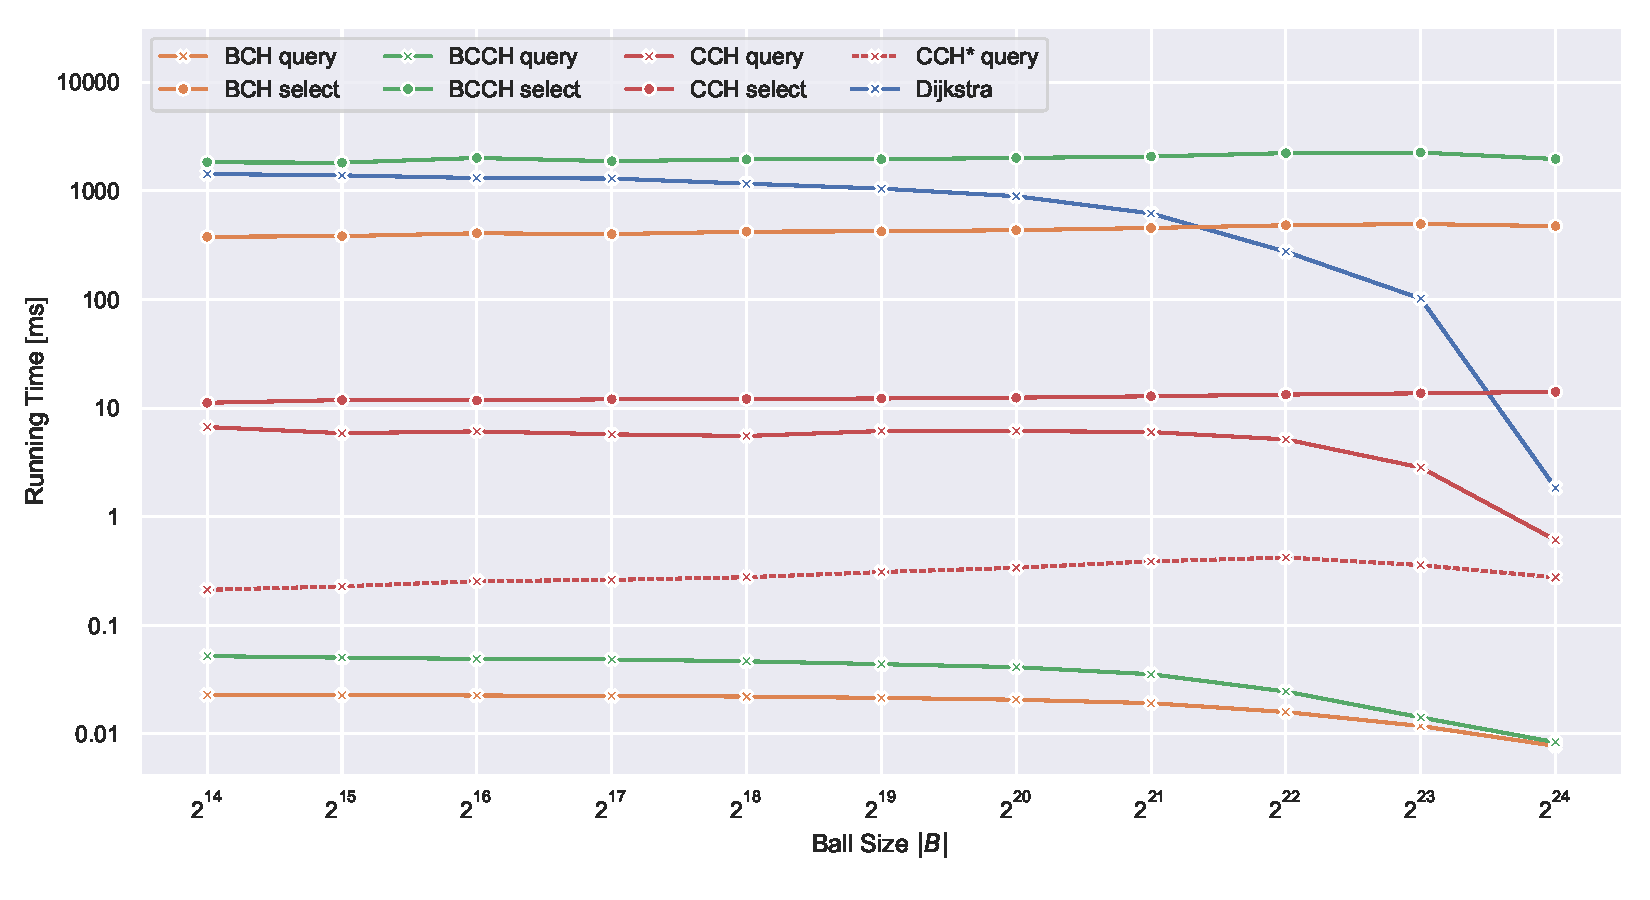
\includegraphics[width=\linewidth]{fig/knn_ball_size.pdf}
\caption{
Selection and query times of various closest-POI algorithms with $|P| = 2^{14}$ POIs picked at random from a ball of varying size $|B|$.
Queries find the $k = 4$ closest POIs.
}\label{fig:knn_ball_size}
\end{figure}

\begin{figure}
\centering
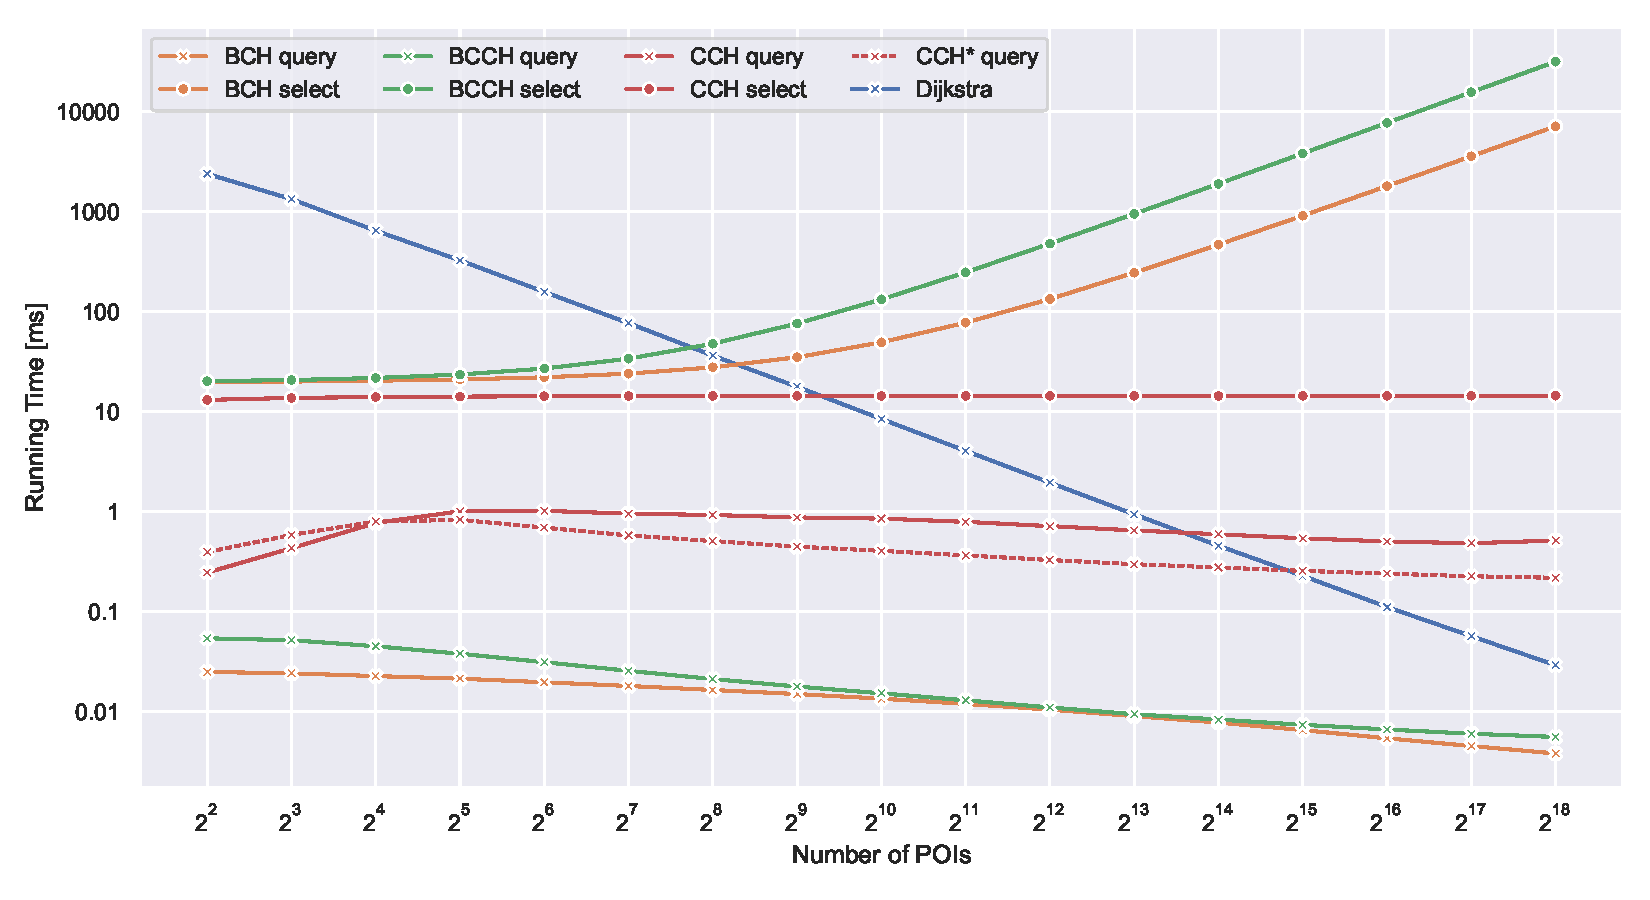
\includegraphics[width=\linewidth]{fig/knn_num_pois.pdf}
\caption{
Selection and query times of various closest-POI algorithms with a varying number $|P|$ of POIs picked at random from a ball of size $|B| = |V|$.
Queries find the $k = 4$ closest POIs.
}\label{fig:knn_num_pois}
\end{figure}

\begin{figure}
\centering
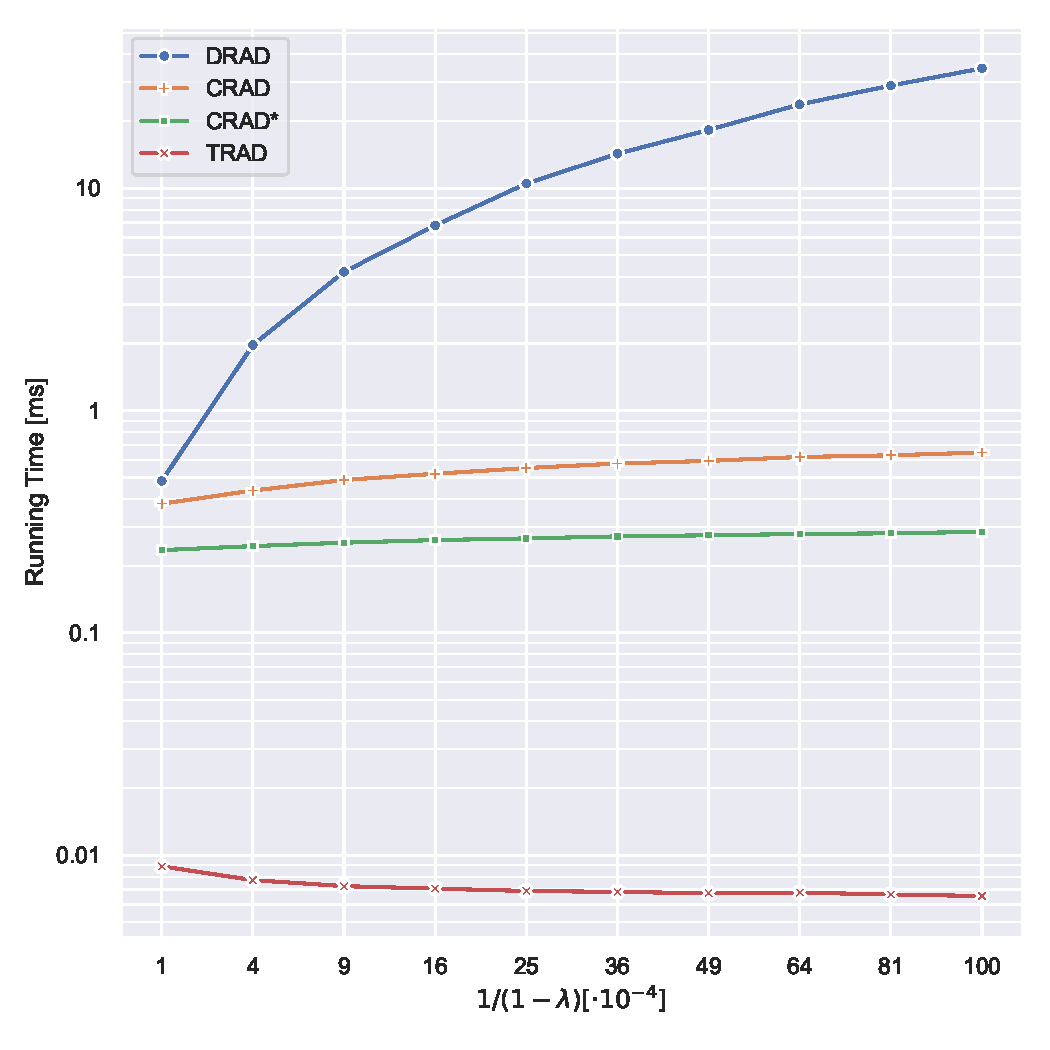
\includegraphics[width=.6363\linewidth]{fig/knn_demands.pdf}
\caption{
Time to generate a single trip with different demand generators for various values of $\lambda$.
}\label{fig:knn_demands}
\end{figure}

\section{Extended Experimental Results on Bidrectional A*}

\begin{table}
\centering
\caption{
Performance of different direction selection criteria of bidirectional A* on OSM Ger with different query weights.
The symmetric variant uses the improved pruning, the average variant does not.
All variants use all low degree optimizations.
}\label{tab:bidir_switching}
\begin{tabular}{cccrrrrrrrr}
\toprule
 &  &  & \multicolumn{5}{c}{Running time [ms]} & \multicolumn{3}{c}{Queue pushs [$\cdot 10^3$]} \\ \cmidrule(lr){4-8} \cmidrule(lr){9-11}\multirow{2}{*}{$w_q$} & Bidirectional & Choose    & \multirow{2}{*}{Zero} & \multirow{2}{*}{ALT} & \multirow{2}{*}{CH} & \multirow{2}{*}{CCH} & \multirow{2}{*}{Oracle} & \multirow{2}{*}{Zero} & \multirow{2}{*}{ALT} & (C)CH/ \\
 & Potential     & Direction & & & & & & & & Oracle \\
\midrule
\multirow{4}{*}{$w_{\ell}$} &   Average &               Alternating &            373.18 & 12.83 &  0.79 &  1.13 &   0.18 &                     916.15 &  23.08 &         0.60 \\
           &   Average &                  Min. Key &            406.35 & 13.68 &  1.44 &  1.75 &   0.56 &                     986.40 &  26.39 &         1.15 \\
           & Symmetric &               Alternating &            376.72 & 40.19 &  0.69 &  0.92 &   0.19 &                     908.55 &  76.61 &         0.57 \\
           & Symmetric &                  Min. Key &            427.51 & 50.46 &  1.77 &  1.99 &   0.83 &                     978.62 &  99.62 &         1.44 \\
\addlinespace
     \multirow{4}{*}{$w_{\ell} \cdot 1.05$} &   Average &               Alternating &            365.82 & 33.22 & 19.34 & 18.66 &   9.96 &                     916.15 &  57.27 &        23.60 \\
           &   Average &                  Min. Key &            391.70 & 38.06 & 21.76 & 20.44 &  11.30 &                     986.41 &  67.65 &        26.42 \\
           & Symmetric &               Alternating &            368.94 & 72.67 & 21.54 & 20.39 &  11.22 &                     908.55 & 123.77 &        20.72 \\
           & Symmetric &                  Min. Key &            394.38 & 84.84 & 27.28 & 24.64 &  14.53 &                     978.63 & 145.28 &        24.82 \\
\addlinespace
   \multirow{4}{*}{\shortstack{$w_{\ell} \cdot 1.5$ if\\ $v <$ 80kph}} &   Average &               Alternating &            361.83 & 19.50 & 10.92 & 10.94 &   5.34 &                     845.06 &  34.03 &        13.25 \\
           &   Average &                  Min. Key &            391.47 & 31.65 & 21.05 & 20.10 &  11.00 &                     917.13 &  52.23 &        23.78 \\
           & Symmetric &               Alternating &            364.55 & 37.33 & 11.89 & 11.75 &   6.00 &                     836.44 &  57.93 &        11.53 \\
           & Symmetric &                  Min. Key &            395.04 & 54.90 & 23.36 & 22.48 &  12.54 &                     908.12 &  84.33 &        22.01 \\
\bottomrule
\end{tabular}


\end{table}

\end{document}
